\chapter{圖的表示、BFS 與 DFS}
\label{ch:gtr}

% 本章的圖共用的樣式（前綴 gtr-）
\tikzset{
    gtr-v/.style={circle, draw=black!70, thick, minimum size=0.62cm, inner sep=0pt, font=\small, fill=white},
    gtr-vs/.style={gtr-v, minimum size=0.5cm, font=\scriptsize},
    gtr-vA/.style={gtr-v, draw=coreStroke, fill=coreFill},
    gtr-vB/.style={gtr-v, draw=memStroke, fill=memFill},
    gtr-e/.style={draw=black!65, thick},
    gtr-a/.style={-{Stealth[length=2.2mm]}, draw=black!65, thick},
    gtr-tree/.style={draw=coreStroke, very thick},
    gtr-treea/.style={gtr-tree, -{Stealth[length=2.4mm]}},
    gtr-back/.style={draw=memStroke, thick, dashed, -{Stealth[length=2.2mm]}},
    gtr-fwd/.style={draw=greenStroke, thick, densely dotted, -{Stealth[length=2.2mm]}},
    gtr-cross/.style={draw=optStroke, thick, dash dot, -{Stealth[length=2.2mm]}},
    gtr-non/.style={draw=black!45, thick, dashed},
    gtr-odd/.style={draw=examStroke, very thick},
    gtr-t/.style={font=\scriptsize, text=black!70, inner sep=1pt},
    gtr-k/.style={font=\scriptsize\bfseries, inner sep=1pt, fill=white},
    gtr-lvl/.style={font=\scriptsize, text=black!55, anchor=east},
    gtr-cell/.style={rectangle, draw=black!65, minimum height=0.5cm, minimum width=0.55cm, inner sep=1pt, font=\small},
    gtr-ptr/.style={-{Stealth[length=1.8mm]}, draw=black!70},
    gtr-iv/.style={draw=coreStroke, fill=coreFill, rounded corners=1pt},
}
% 虛擬碼裡的三種顏色
\newcommand{\gtrwhite}{\textsc{white}}
\newcommand{\gtrgray}{\textsc{gray}}
\newcommand{\gtrblack}{\textsc{black}}
% 鄰接串列的一列：\gtradjrow{y}{頂點}{鄰居串列（逗號分開，空的寫 {}）}
\newcommand{\gtradjrow}[3]{%
    \node[gtr-cell, minimum width=0.7cm] (h#2) at (0, #1) {#2};
    \def\gtrprev{h#2}%
    \foreach \gtrv [count=\gtrk] in {#3} {
        \node[gtr-cell] (n#2-\gtrk) at (0.6 + \gtrk*1.05, #1) {\gtrv};
        \draw[gtr-ptr] (\gtrprev.east) -- (n#2-\gtrk.west);
        \xdef\gtrprev{n#2-\gtrk}%
    }
    \node[font=\scriptsize, anchor=west, text=black!60] at (\gtrprev.east) {\,\NIL};
}

登山社把後山的步道畫成一張圖：岔路口和景點是點，兩點之間有一段步道就連一條線。 新
社員從停車場出發，想知道到每個景點最少要走幾段步道；社長想知道地圖上有沒有哪些點從
停車場根本走不到。 社團網站也可以畫成類似的圖：每一頁是一個點，頁面上有連到另一頁的
超連結，就畫一個從這頁指向那頁的箭頭；管理員想知道，一直點連結會不會繞回同一頁。 這
幾件事都要把圖有系統地走一遍。 如果讓你拿著地圖一個點一個點去標記，你會照什麼順序走，
才能保證每個走得到的點都標到、而且不重複？ 往下讀之前，先想一想。

這一章是第五部「圖論」的第一章。 先把圖的名詞和符號定下來，第~22~到~26~章都沿用這一
套；接著講兩種存圖的方法，再講兩種走訪圖的方法。 \textbf{廣度優先搜尋}（breadth-first
search，BFS）從起點一圈一圈往外擴，順便求出到每個點最少要走幾條邊；\textbf{深度優先搜
尋}（depth-first search，DFS）沿著一條路走到底，走不下去才退回上一個岔路口，它留下的
「發現時間」和「完成時間」可以把圖的邊分成四類。 第~22~章的拓樸排序、第~23~章的強連
通元件和割點，都建立在這些時間上。 最後用兩種搜尋解三個問題：連通元件、二分圖、有向
環。

這一章用到《C 程式設計基礎》第~14~章的結構指標、第~15~章的遞迴，以及第~19~章的
\texttt{malloc}、指標的指標和串列。 本書第~5~章的串列插入、第~6~章的佇列和堆疊、
第~7~章的樹和層序走訪、第~13~章的互斥集合都只引用，不再重講。

\section{圖的名詞與符號}
\label{sec:gtr-terms}

\subsection{圖、頂點、邊}

一張\textbf{圖}（graph）寫成 $G = (V, E)$。 $V$ 是有限個\textbf{頂點}（vertex，也
叫節點）組成的集合，$E$ 是\textbf{邊}（edge）組成的集合，每條邊連接兩個頂點。 本書
用
\[
n = |V|, \qquad m = |E|
\]
表示頂點數和邊數，演算法的時間寫成 $n$ 和 $m$ 的函數，例如 $\Theta(n + m)$。

\begin{itemize}
\item \textbf{無向圖}（undirected graph）的邊沒有方向。 連接 $u$、$v$ 的邊是集合
$\{u, v\}$，習慣上也寫成 $(u, v)$，這時 $(u, v)$ 和 $(v, u)$ 是同一條邊。 步道圖是無
向圖：一段步道兩個方向都能走。
\item \textbf{有向圖}（directed graph）的邊有方向。 邊 $(u, v)$ 是有序對，畫成從 $u$
指向 $v$ 的箭頭，也寫成 $u \to v$；$u$ 叫這條邊的\textbf{尾}（tail），$v$ 叫\textbf{頭}
（head）。 $(u, v)$ 和 $(v, u)$ 是兩條不同的邊，可以只有其中一條。 網頁的超連結是有向
圖：$A$ 頁連到 $B$ 頁，不代表 $B$ 頁也連回 $A$。
\end{itemize}

兩端是同一個頂點的邊 $(v, v)$ 叫\textbf{自環}（self-loop）；同一對頂點之間不只一條邊，
叫\textbf{重邊}（multiple edges）。 沒有自環也沒有重邊的圖叫\textbf{簡單圖}（simple
graph）。 \textbf{本書第~21~到~26~章的圖，除非特別說明，都是簡單圖}：無向圖每一對頂點
之間最多一條邊；有向圖沒有自環，從 $u$ 到 $v$ 最多一條邊（$u \to v$ 和 $v \to u$ 可以
同時存在，它們是不同的兩條）。

如果 $(u, v) \in E$，就說 $v$ 和 $u$ \textbf{相鄰}（adjacent），$v$ 是 $u$ 的一個
\textbf{鄰居}（neighbor），而邊 $(u, v)$ 和頂點 $u$、$v$ \textbf{關聯}（incident）。 在
有向圖裡，「$v$ 是 $u$ 的鄰居」只看從 $u$ 出去的邊：$u \to v$ 存在時 $v$ 是 $u$ 的鄰居，
反過來不一定。

圖~\ref{fig:gtr-examples} 是本章一直會用到的兩張圖。 左邊的 $G_1$ 是步道圖，十個頂點用
$1$ 到 $10$ 編號，$1$ 是停車場；$8$、$9$、$10$ 在溪的對岸，和其他點之間沒有步道。 右邊
的 $G_2$ 是社團網站的八個頁面，用大寫字母 $A$ 到 $H$ 命名。 頂點的名字在虛擬碼和手算
裡用 $1..n$ 或字母，在 C 程式裡一律換成 $0..n-1$：頂點 $i$ 存成 \texttt{i - 1}，字母
$X$ 存成 \texttt{X - 'A'}，印出來時再換回去。

\begin{center}
\begin{tikzpicture}[x=1cm, y=1cm]
\begin{scope}
\node[gtr-v] (u1) at (0, 0) {1};
\node[gtr-v] (u2) at (1.5, 1) {2};
\node[gtr-v] (u3) at (1.5, -1) {3};
\node[gtr-v] (u4) at (3, 1) {4};
\node[gtr-v] (u5) at (3, -1) {5};
\node[gtr-v] (u6) at (4.5, 1) {6};
\node[gtr-v] (u7) at (4.5, -1) {7};
\node[gtr-v] (u8) at (6, 1) {8};
\node[gtr-v] (u9) at (6, 0) {9};
\node[gtr-v] (u10) at (6, -1) {10};
\foreach \a/\b in {1/2, 1/3, 2/4, 3/4, 3/5, 4/6, 5/6, 5/7, 6/7, 8/9, 9/10}
    \draw[gtr-e] (u\a) -- (u\b);
\node[font=\small] at (3, -1.9) {$G_1$：步道（無向）};
\end{scope}
\begin{scope}[xshift=7.6cm]
\node[gtr-v] (A) at (0, 0) {$A$};
\node[gtr-v] (B) at (1.6, 1) {$B$};
\node[gtr-v] (C) at (3.2, 1) {$C$};
\node[gtr-v] (E) at (1.6, -1) {$E$};
\node[gtr-v] (D) at (3.2, -1) {$D$};
\node[gtr-v] (G) at (4.8, 1) {$G$};
\node[gtr-v] (F) at (4.8, -1) {$F$};
\node[gtr-v] (H) at (6.2, 0) {$H$};
\draw[gtr-a] (A) -- (B);
\draw[gtr-a] (B) -- (C);
\draw[gtr-a] (C) to[bend right=38] (A);
\draw[gtr-a] (A) -- (E);
\draw[gtr-a] (B) -- (E);
\draw[gtr-a] (E) -- (D);
\draw[gtr-a] (D) -- (C);
\draw[gtr-a] (A) to[bend right=38] (D);
\draw[gtr-a] (F) -- (G);
\draw[gtr-a] (G) -- (C);
\draw[gtr-a] (G) -- (H);
\draw[gtr-a] (F) to[bend left=12] (H);
\draw[gtr-a] (H) to[bend left=12] (F);
\node[font=\small] at (3.1, -2.2) {$G_2$：網站的頁面（有向）};
\end{scope}
\end{tikzpicture}
\diagcaption{本章的兩張例子圖。 $G_1$ 有 $n = 10$、$m = 11$；$G_2$ 有 $n = 8$、$m = 13$。
$G_2$ 的 $F$ 和 $H$ 之間兩個方向各有一條邊。}
\label{fig:gtr-examples}
\end{center}

\subsection{度數}

無向圖裡，和頂點 $v$ 關聯的邊數叫 $v$ 的\textbf{度數}（degree），寫成 $\deg(v)$。 有向
圖分成兩個：從 $v$ 出去的邊數叫\textbf{出度}（out-degree）$\deg^{+}(v)$，指進 $v$ 的邊
數叫\textbf{入度}（in-degree）$\deg^{-}(v)$。 有些課本把度數叫「分支度」，入度、出度
叫「內分支度」「外分支度」；第~7~章樹的「分支度」是子節點個數，和這裡的度數不一樣（樹
當成無向圖時，非根節點的度數是子節點數加 $1$）。

在 $G_1$ 裡，$\deg(3) = \deg(5) = \deg(6) = 3$，$\deg(8) = 1$；在 $G_2$ 裡，
$\deg^{+}(A) = 3$、$\deg^{-}(A) = 1$，$\deg^{+}(C) = 1$、$\deg^{-}(C) = 3$。

\begin{theorem}[握手定理]
\label{thm:gtr-handshake}
無向圖裡 $\displaystyle\sum_{v \in V} \deg(v) = 2m$。 有向圖裡
$\displaystyle\sum_{v \in V} \deg^{+}(v) = \sum_{v \in V} \deg^{-}(v) = m$。
\end{theorem}

\begin{proof}
無向圖的每條邊 $\{u, v\}$ 在 $\deg(u)$ 和 $\deg(v)$ 各算一次，所以每條邊在左邊的和裡剛
好算兩次。 有向圖的每條邊 $(u, v)$ 只在 $\deg^{+}(u)$ 算一次，也只在 $\deg^{-}(v)$ 算一
次。
\end{proof}

一個馬上得到的結果：無向圖裡度數是奇數的頂點有偶數個，因為所有度數加起來是偶數。
$G_1$ 的度數依序是 $2, 2, 3, 3, 3, 3, 2, 1, 2, 1$，和是 $22 = 2 \times 11$，奇數度數的
頂點有 $3, 4, 5, 6, 8, 10$ 共六個。

邊數有上界。 $n$ 個頂點的簡單無向圖，每一對頂點最多一條邊，所以
$m \le \binom{n}{2} = n(n-1)/2$；簡單有向圖每個有序對最多一條邊，$m \le n(n-1)$。 每一
對頂點之間都有邊的無向圖叫\textbf{完全圖}（complete graph），寫成 $K_n$。 所以
$m = O(n^2)$，$\lg m = O(\lg n)$。 $m$ 遠小於 $n^2$ 的圖叫\textbf{稀疏}（sparse）圖，
$m$ 接近 $n^2$ 的叫\textbf{稠密}（dense）圖。 道路、網頁、社群關係這類實際的圖大多很稀
疏，這是下一節選擇存法的主要考量。

\subsection{路徑與環}

\begin{definition}[路徑]
\label{def:gtr-path}
從 $u$ 到 $v$ 的一條\textbf{路徑}（path）是一串頂點 $\langle v_0, v_1, \ldots, v_k
\rangle$，其中 $v_0 = u$、$v_k = v$，而且 $(v_{i-1}, v_i) \in E$，$i = 1, 2, \ldots,
k$。 $k$ 是路徑的\textbf{長度}，也就是經過的邊數；只有一個頂點的 $\langle u \rangle$ 是
長度 $0$ 的路徑。 路徑上的頂點都不相同時，叫\textbf{簡單路徑}（simple path）。
\end{definition}

有向圖的路徑要順著箭頭走。 從 $u$ 到 $v$ 有路徑時，說 $v$ 從 $u$ \textbf{可到達}
（reachable），寫成 $u \leadsto v$。 例如 $G_2$ 裡 $\langle F, G, C, A, B \rangle$ 是長
度 $4$ 的簡單路徑，所以 $F \leadsto B$；但從 $A$ 出發的路徑都到不了 $F$。

路徑可以重複經過頂點，例如 $G_1$ 的 $\langle 1, 2, 4, 3, 1, 2 \rangle$。 如果從 $u$ 到
$v$ 有路徑，就一定有簡單路徑：路徑上某個頂點 $x$ 出現兩次時，把兩次之間繞的那一圈剪
掉，還是從 $u$ 到 $v$ 的路徑，而且比較短；一直剪到沒有重複為止。 所以談「可不可以到
達」「最短路徑」時，只要考慮簡單路徑。

\begin{definition}[環]
\label{def:gtr-cycle}
\textbf{環}（cycle）是一條長度 $k \ge 1$、起點等於終點（$v_0 = v_k$）的路徑，而且
$v_1, v_2, \ldots, v_k$ 互不相同。 無向圖另外要求 $k \ge 3$。 沒有環的圖叫\textbf{無環}
（acyclic）。
\end{definition}

無向圖要求 $k \ge 3$，是為了排除 $\langle u, v, u \rangle$ 這種沿著同一條邊走過去再走回
來的情形。 有向圖的 $\langle u, v, u \rangle$ 用到 $u \to v$ 和 $v \to u$ 兩條不同的邊，
是長度 $2$ 的環，例如 $G_2$ 的 $\langle F, H, F \rangle$。 $G_2$ 的另一個環是
$\langle A, B, C, A \rangle$；$G_1$ 有 $\langle 5, 6, 7, 5 \rangle$、
$\langle 1, 2, 4, 3, 1 \rangle$ 等好幾個環。

沒有環的有向圖叫\textbf{有向無環圖}（directed acyclic graph，DAG）。 先修課程、工程
的先後順序都是 DAG，第~22~章的拓樸排序就在 DAG 上做。

\begin{examnote}
路徑和環的定義，各本書不太一樣。 有的書說的「路徑」就是本書的簡單路徑，另外用
walk 或「通路」稱呼可以重複頂點的走法；有的書把本書的環叫「簡單環」，「環」則允許重
複頂點。 另外，有些課本把有向邊寫成 $\langle u, v \rangle$、無向邊寫成 $(u, v)$ 來區分。
題目問「有幾條路徑」「最長的環」這類會因定義而不同的問題時，先看題目怎麼定義；題目沒
給，就在答案開頭寫一句你用的定義。
\end{examnote}

\subsection{連通}

無向圖裡，如果任兩個頂點之間都有路徑，這張圖叫\textbf{連通}（connected）。 不連通
的圖會分成好幾塊：在無向圖裡，「$u$ 和 $v$ 之間有路徑」滿足自反（長度 $0$ 的路徑）、
對稱（路徑倒過來走）和遞移（兩條路徑接起來），是一個等價關係，它的每一個等價類叫一個
\textbf{連通元件}（connected component，也叫連通分量）。 每個連通元件內部是連通的，
不同元件之間沒有邊。 $G_1$ 有兩個連通元件 $\{1, 2, \ldots, 7\}$ 和 $\{8, 9, 10\}$。
第~13~章的互斥集合處理的就是這種「誰和誰同一塊」的問題，第~\ref{sec:gtr-app}~節會比較
兩種做法。

有向圖的「可到達」沒有對稱性：$G_2$ 裡 $F \leadsto A$，但 $A$ 到不了 $F$。 如果有向圖裡
任兩個頂點 $u$、$v$ 都有 $u \leadsto v$ 而且 $v \leadsto u$，這張圖叫\textbf{強連通}
（strongly connected）。 「互相可達」又是一個等價關係，它的等價類叫\textbf{強連通元
件}（strongly connected component）。 $G_2$ 的強連通元件是 $\{A, B, C, D, E\}$、
$\{F, G, H\}$：$A$ 到 $E$ 這五頁可以互相點過去，$F$、$G$、$H$ 也是，但兩組之間只有從
$G$ 到 $C$ 的單向連結。 強連通元件怎麼有效率地求出來，是第~23~章的主題；把有向邊都當
成無向邊之後連通的有向圖，叫\textbf{弱連通}（weakly connected）。

\subsection{子圖、樹與生成樹}

$G' = (V', E')$ 是 $G = (V, E)$ 的\textbf{子圖}（subgraph），如果 $V' \subseteq V$、
$E' \subseteq E$，而且 $E'$ 的每條邊兩端都在 $V'$ 裡。 $V' = V$ 的子圖叫\textbf{生成子
圖}（spanning subgraph），也就是頂點全留、邊挑一部分。 給一個頂點集合 $V'$，把 $E$ 裡
兩端都在 $V'$ 的邊全部留下來，得到的子圖叫 $V'$ 的\textbf{誘導子圖}（induced
subgraph），寫成 $G[V']$。 例如 $G_1[\{5, 6, 7\}]$ 是一個三角形。

連通而且無環的無向圖叫\textbf{樹}（tree），每個連通元件都是樹的無向圖（也就是無環的無
向圖）叫\textbf{森林}（forest）。 這裡的樹沒有指定根，也叫自由樹（free tree）；挑一個頂
點當根，從根往外看，就得到第~7~章的有根樹。

下面的引理把邊數、連通元件數和環連在一起，後面好幾個地方會用到。

\begin{lemma}
\label{lem:gtr-count}
$n$ 個頂點、$m$ 條邊的無向圖至少有 $n - m$ 個連通元件，而且剛好 $n - m$ 個的充分必要
條件是這張圖沒有環。
\end{lemma}

\begin{proof}
從 $n$ 個孤立的頂點開始（$n$ 個元件），把 $m$ 條邊一條一條加進去。 加入邊 $(u, v)$ 時
有兩種情形：
\begin{itemize}
\item $u$、$v$ 原本就在同一個元件：元件數不變。 原本已經有一條 $u$ 到 $v$ 的簡單路徑，
再加上這條邊就形成一個環。
\item $u$、$v$ 原本在不同元件：兩個元件併成一個，元件數減一。
\end{itemize}
每條邊最多讓元件數減一，所以最後至少剩 $n - m$ 個。 剛好剩 $n - m$ 個，等於說每條邊都
屬於第二種情形。 如果某條邊屬於第一種，最後的圖顯然有環；反過來，如果最後的圖有環，看
這個環上最後加入的那條邊 $(u, v)$，加入它的時候，環上其他的邊已經把 $u$、$v$ 連起來
了，它屬於第一種情形。
\end{proof}

這個證明和第~13~章用互斥集合數連通元件是同一件事：每一次真正的合併讓集合數減一，兩
端已經在同一組的邊不改變集合數，而且正好是會造成環的邊（第~24~章的 Kruskal 演算法就
靠這一點挑邊）。 由引理~\ref{lem:gtr-count} 可以得到樹的幾種等價說法。

\begin{theorem}
\label{thm:gtr-tree}
$G$ 是 $n$ 個頂點、$m$ 條邊的無向圖。 下面四句話互相等價：
\begin{enumerate}
\item $G$ 是樹（連通而且無環）。
\item $G$ 連通，而且 $m = n - 1$。
\item $G$ 無環，而且 $m = n - 1$。
\item $G$ 的任兩個頂點之間剛好有一條簡單路徑。
\end{enumerate}
\end{theorem}

\begin{proof}
連通表示元件數是 $1$。 (1)$\Rightarrow$(2)：無環，由引理元件數等於 $n - m$，又等於
$1$，所以 $m = n - 1$。 (2)$\Rightarrow$(3)：元件數 $1 = n - m$，引理的等號成立，所以
無環。 (3)$\Rightarrow$(1)：無環，元件數 $= n - m = 1$，所以連通。 (1)$\Rightarrow$(4)：
連通保證至少一條簡單路徑；如果 $u$ 到 $v$ 有兩條不同的簡單路徑，從 $u$ 出發，找到兩條第
一次分岔的地方和之後第一次再碰頭的地方，兩段合起來是一個環，矛盾。 (4)$\Rightarrow$
(1)：有路徑所以連通；如果有環 $\langle v_0, \ldots, v_k = v_0 \rangle$，$v_0$ 到 $v_1$ 就
有兩條簡單路徑（直接走邊，或沿著環的另一邊繞過去，$k \ge 3$ 保證這是不同的路徑），矛
盾。
\end{proof}

無向圖 $G$ 的\textbf{生成樹}（spanning tree）是一個生成子圖，而且是一棵樹：$n$ 個頂點
全部留下，挑 $n - 1$ 條邊把它們連起來。 $G$ 有生成樹的充分必要條件是 $G$ 連通。 不連
通的圖，每個連通元件各取一棵生成樹，合起來叫\textbf{生成森林}。 這一章的 BFS 和 DFS 都
會順手產生一棵生成樹（或生成森林）；第~24~章要找的，是邊上有權重時總權重最小的那一棵。

\textbf{加權圖}（weighted graph）是每條邊 $(u, v)$ 另外帶一個數 $w(u, v)$ 的圖，例如步
道的長度、網路連線的費用。 這一章的圖都不帶權重，「最短」指的是邊數最少；第~24~到~26~
章再處理權重。

下表整理本章定下的符號，第~22~到~26~章照用。

\begin{center}
\begin{tabular}{lll}
\toprule
符號 & 意思 & 備註 \\
\midrule
$G = (V, E)$ & 圖、頂點集合、邊集合 & \\
$n = |V|$，$m = |E|$ & 頂點數、邊數 & 時間寫成 $\Theta(n + m)$ \\
$(u, v)$，$u \to v$ & 邊；有向圖是從 $u$ 到 $v$ & 無向圖的 $(u, v)$ 就是 $\{u, v\}$ \\
$\deg(v)$ & 無向圖的度數 & $\sum \deg(v) = 2m$ \\
$\deg^{+}(v)$，$\deg^{-}(v)$ & 有向圖的出度、入度 & 和都是 $m$ \\
$u \leadsto v$ & 從 $u$ 可以到達 $v$ & 有長度 $\ge 0$ 的路徑 \\
$\delta(u, v)$ & 從 $u$ 到 $v$ 最少要走幾條邊 & 到不了是 $\infty$（第~\ref{sec:gtr-bfs}~節） \\
$\mathit{Adj}[u]$ & $u$ 的鄰接串列 & 第~\ref{sec:gtr-repr}~節 \\
$d[v]$，$\pi[v]$ & BFS 的距離、前驅 & 到不了是 $\infty$、\NIL \\
$d[v]$，$f[v]$ & DFS 的發現、完成時間 & 從 $1$ 起，共 $2n$ 個時間 \\
白、灰、黑 & 頂點的狀態（\gtrwhite、\gtrgray、\gtrblack）& 第~\ref{sec:gtr-bfs}、\ref{sec:gtr-dfs}~節 \\
\bottomrule
\end{tabular}
\end{center}

\section{圖的表示法}
\label{sec:gtr-repr}

演算法要問圖的問題，最常見的是兩種：「$(u, v)$ 是不是一條邊？」和「$u$ 的鄰居有哪
些？」。 兩種標準存法各自讓其中一種問題比較快。

\subsection{鄰接矩陣}

頂點編號成 $1..n$ 之後，\textbf{鄰接矩陣}（adjacency matrix）是一個 $n \times n$ 的
矩陣 $A = (a_{uv})$：
\[
a_{uv} = \begin{cases} 1, & (u, v) \in E, \\ 0, & \text{其他}. \end{cases}
\]
下表是 $G_2$ 的鄰接矩陣，第 $u$ 列第 $v$ 行是 $1$ 表示有 $u \to v$ 這條邊。

\begin{center}
\begin{tabular}{c|cccccccc|c}
 & $A$ & $B$ & $C$ & $D$ & $E$ & $F$ & $G$ & $H$ & 列和 $= \deg^{+}$ \\
\hline
$A$ & 0 & 1 & 0 & 1 & 1 & 0 & 0 & 0 & 3 \\
$B$ & 0 & 0 & 1 & 0 & 1 & 0 & 0 & 0 & 2 \\
$C$ & 1 & 0 & 0 & 0 & 0 & 0 & 0 & 0 & 1 \\
$D$ & 0 & 0 & 1 & 0 & 0 & 0 & 0 & 0 & 1 \\
$E$ & 0 & 0 & 0 & 1 & 0 & 0 & 0 & 0 & 1 \\
$F$ & 0 & 0 & 0 & 0 & 0 & 0 & 1 & 1 & 2 \\
$G$ & 0 & 0 & 1 & 0 & 0 & 0 & 0 & 1 & 2 \\
$H$ & 0 & 0 & 0 & 0 & 0 & 1 & 0 & 0 & 1 \\
\hline
行和 $= \deg^{-}$ & 1 & 1 & 3 & 2 & 2 & 1 & 1 & 2 & 13 \\
\end{tabular}
\end{center}

從定義直接看得出幾件事：
\begin{itemize}
\item 第 $u$ 列的和是 $\deg^{+}(u)$，第 $v$ 行的和是 $\deg^{-}(v)$，全部的 $1$ 共有 $m$ 個。
\item 無向圖的鄰接矩陣是對稱的（$a_{uv} = a_{vu}$），$1$ 共有 $2m$ 個；沒有自環時對角線
全是 $0$。 對稱矩陣只要存下三角的 $n(n-1)/2$ 格，位址怎麼算見第~4~章的三角矩陣壓縮。
\item 判斷 $(u, v)$ 是不是邊只要讀一格，$\Theta(1)$；列出 $u$ 的所有鄰居要把第 $u$ 列
整列掃過，$\Theta(n)$，不管 $u$ 實際上有幾個鄰居。
\item 不管邊有多少，都要 $\Theta(n^2)$ 的空間，光是把矩陣設成 $0$ 就要 $\Theta(n^2)$ 的
時間。 $n = 10^5$ 的道路圖，即使每格只用一個位元，也要大約 $1.25 \times 10^9$ 位元
組。
\end{itemize}

加權圖的鄰接矩陣在 $a_{uv}$ 存權重 $w(u, v)$，沒有邊的格子存一個代表「沒有邊」的值，
最短路徑問題通常存 $\infty$。 第~25~章的 Floyd--Warshall 演算法直接在這種矩陣上計算。

\subsection{鄰接串列}

\textbf{鄰接串列}（adjacency list）用一個長度 $n$ 的陣列 $\mathit{Adj}[1..n]$，
$\mathit{Adj}[u]$ 是一條串列，存 $u$ 的所有鄰居。 圖~\ref{fig:gtr-adjlist} 是 $G_1$ 的鄰
接串列。 有向圖的 $\mathit{Adj}[u]$ 只存從 $u$ 出去的邊的另一端；無向圖的每條邊
$\{u, v\}$ 要存兩次，$v$ 在 $\mathit{Adj}[u]$ 裡，$u$ 也在 $\mathit{Adj}[v]$ 裡。

\begin{center}
\begin{tikzpicture}[x=1cm, y=0.62cm]
\gtradjrow{0}{1}{2,3}
\gtradjrow{-1}{2}{1,4}
\gtradjrow{-2}{3}{1,4,5}
\gtradjrow{-3}{4}{2,3,6}
\gtradjrow{-4}{5}{3,6,7}
\gtradjrow{-5}{6}{4,5,7}
\gtradjrow{-6}{7}{5,6}
\gtradjrow{-7}{8}{9}
\gtradjrow{-8}{9}{8,10}
\gtradjrow{-9}{10}{9}
\node[font=\scriptsize, text=black!60] at (0, 0.75) {$\mathit{Adj}$};
\end{tikzpicture}
\diagcaption{$G_1$ 的鄰接串列。 左邊一格是陣列 $\mathit{Adj}$ 的一個元素，存那條串列的
第一個節點；每條串列裡的鄰居由小到大排。 $11$ 條邊，共 $22$ 個節點。}
\label{fig:gtr-adjlist}
\end{center}

串列節點總數是 $m$（有向）或 $2m$（無向），加上陣列的 $n$ 格，空間是 $\Theta(n + m)$。
列出 $u$ 的所有鄰居花 $\Theta(1 + \deg(u))$，只和 $u$ 實際的鄰居數有關；代價是判斷
$(u, v)$ 是不是邊時要在 $\mathit{Adj}[u]$ 裡一個一個找，最壞 $\Theta(\deg(u))$。

同一張圖的鄰接串列不只一種，串列裡的順序可以任意排。 BFS 和 DFS 走的順序就是串列的順
序，所以順序不同，走出來的結果也不同。 \textbf{本書的約定：每條串列裡的鄰居按編號（或
字母）由小到大排}，手算追蹤和 C 程式都照這個順序。

有向圖的鄰接串列只記出去的邊，要知道「誰指向 $v$」得把整個結構掃一遍。 需要常常查入
邊時（例如第~22~章 Kahn 演算法要的入度、第~23~章要的轉置圖），可以另外建一份\textbf{反
鄰接串列}（inverse adjacency list）：$\mathit{Adj}^{-1}[v]$ 存所有 $u \to v$ 的 $u$。
它其實就是把每條邊反過來的圖（轉置圖）的鄰接串列。

\subsection{其他幾種存法}

下面三種存法在資料結構課本和考題裡常見，這裡只講結構，本書後面的程式不會用到。

\textbf{邊串列}（edge list）。 用一個長度 $m$ 的陣列存每條邊的兩端（加權時再存權
重），空間 $\Theta(m)$。 它不能快速列出鄰居，但「把所有邊依權重排序」很方便，第~13~章
的互斥集合和第~24~章的 Kruskal 演算法都直接吃邊串列。

\textbf{循序表示}（也叫壓縮鄰接陣列）。 圖建好之後不再改變時，可以把所有鄰接串列依頂點
順序接成一個長度 $m$（無向圖是 $2m$）的陣列 $\mathit{nbr}$，另外用陣列
$\mathit{start}[1..n+1]$ 記每個頂點的鄰居從哪一格開始：$u$ 的鄰居是
$\mathit{nbr}[\mathit{start}[u] .. \mathit{start}[u+1] - 1]$，$\mathit{start}[n+1]$ 設成
$m + 1$ 當結尾。 $G_2$ 存成：

\begin{center}
\begin{tabular}{l|ccccccccc}
 & $A$ & $B$ & $C$ & $D$ & $E$ & $F$ & $G$ & $H$ & （結尾）\\
\hline
$\mathit{start}$ & 1 & 4 & 6 & 7 & 8 & 9 & 11 & 13 & 14 \\
\end{tabular}

\smallskip
\begin{tabular}{l|ccccccccccccc}
 & 1 & 2 & 3 & 4 & 5 & 6 & 7 & 8 & 9 & 10 & 11 & 12 & 13 \\
\hline
$\mathit{nbr}$ & $B$ & $D$ & $E$ & $C$ & $E$ & $A$ & $C$ & $D$ & $G$ & $H$ & $C$ & $H$ & $F$ \\
\end{tabular}
\end{center}

$\deg^{+}(u) = \mathit{start}[u+1] - \mathit{start}[u]$，例如 $\deg^{+}(F) = 11 - 9 = 2$。
它和鄰接串列一樣是 $\Theta(n + m)$ 的空間，但沒有指標，資料連續存放，走訪時比較快；缺點
是加一條邊要把後面的資料全部往後搬。

\textbf{鄰接多重串列}（adjacency multilist）。 無向圖的鄰接串列把每條邊存兩次，對邊做
標記（例如「這條邊走過了」）時，兩份都要改。 鄰接多重串列讓每條邊只有一個節點，節點裡
存兩端 $u$、$v$，以及兩個指標：$\mathit{link}_u$ 指向下一條和 $u$ 關聯的邊，
$\mathit{link}_v$ 指向下一條和 $v$ 關聯的邊；需要時再加一個標記欄位。 每個頂點的串列頭
指向第一條和它關聯的邊，沿著「自己那一端」的指標走，就能列出它的所有邊。 下面是一張四
個頂點、五條邊的圖，邊依 $e_1$ 到 $e_5$ 的順序串起來：

\begin{center}
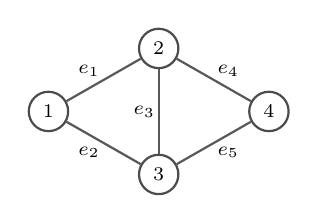
\begin{tikzpicture}[x=1cm, y=1cm, baseline=(current bounding box.center)]
\node[gtr-vs] (m1) at (0, 0) {1};
\node[gtr-vs] (m2) at (1.4, 0.8) {2};
\node[gtr-vs] (m3) at (1.4, -0.8) {3};
\node[gtr-vs] (m4) at (2.8, 0) {4};
\draw[gtr-e] (m1) -- node[gtr-k, above left] {$e_1$} (m2);
\draw[gtr-e] (m1) -- node[gtr-k, below left] {$e_2$} (m3);
\draw[gtr-e] (m2) -- node[gtr-k, left] {$e_3$} (m3);
\draw[gtr-e] (m2) -- node[gtr-k, above right] {$e_4$} (m4);
\draw[gtr-e] (m3) -- node[gtr-k, below right] {$e_5$} (m4);
\end{tikzpicture}
\qquad
\begin{tabular}{cccccc}
\toprule
邊 & $u$ & $v$ & $\mathit{link}_u$ & $\mathit{link}_v$ \\
\midrule
$e_1$ & 1 & 2 & $e_2$ & $e_3$ \\
$e_2$ & 1 & 3 & \NIL & $e_3$ \\
$e_3$ & 2 & 3 & $e_4$ & $e_5$ \\
$e_4$ & 2 & 4 & \NIL & $e_5$ \\
$e_5$ & 3 & 4 & \NIL & \NIL \\
\bottomrule
\end{tabular}
\qquad
\begin{tabular}{cc}
\toprule
頂點 & 串列頭 \\
\midrule
1 & $e_1$ \\
2 & $e_1$ \\
3 & $e_2$ \\
4 & $e_4$ \\
\bottomrule
\end{tabular}
\end{center}

列出頂點 $3$ 的邊：從串列頭 $e_2$ 開始，$3$ 是 $e_2$ 的 $v$ 端，下一條看
$\mathit{link}_v = e_3$；$3$ 是 $e_3$ 的 $v$ 端，下一條是 $e_5$；$3$ 是 $e_5$ 的 $u$ 端，
$\mathit{link}_u = \NIL$，結束。 得到 $e_2, e_3, e_5$。 走的時候每到一個節點都要先看自己
是 $u$ 端還是 $v$ 端，再決定跟哪一個指標。 有向圖也有類似的做法，每條邊一個節點，同時
串在尾端的出邊串列和頭端的入邊串列上，叫\textbf{十字串列}（orthogonal list），就是第~5~
章稀疏矩陣的正交串列用在鄰接矩陣上。

\subsection{比較}

\begin{center}
\begin{tabular}{lcc}
\toprule
操作 & 鄰接矩陣 & 鄰接串列 \\
\midrule
空間 & $\Theta(n^2)$ & $\Theta(n + m)$ \\
判斷 $(u, v)$ 是不是邊 & $\Theta(1)$ & $O(\deg(u))$ \\
列出 $u$ 的所有鄰居 & $\Theta(n)$ & $\Theta(1 + \deg(u))$ \\
掃過所有的邊（BFS、DFS）& $\Theta(n^2)$ & $\Theta(n + m)$ \\
算出所有頂點的入度 & $\Theta(n^2)$ & $\Theta(n + m)$ \\
加一條邊 & $\Theta(1)$ & $\Theta(1)$（插在開頭）\\
刪一條邊 $(u, v)$ & $\Theta(1)$ & $O(\deg(u))$（無向：$+\deg(v)$）\\
\bottomrule
\end{tabular}
\end{center}

圖稀疏時（大部分的實際問題），鄰接串列的空間和走訪時間都好得多，本書的圖演算法預設
用鄰接串列。 鄰接矩陣適合三種情形：圖很稠密，$m$ 本來就接近 $n^2$；演算法需要大量
「$(u, v)$ 是不是邊」的查詢；$n$ 很小，寫起來簡單比較重要。 第~25~章的 Floyd--Warshall
和遞移閉包都用矩陣。

\begin{examnote}
題目只給一張圖、問「用鄰接串列表示」時，串列裡的順序會影響之後 BFS、DFS 的答案。
沒有特別說明時，照本書的約定由小到大排，並在答案裡寫一句「串列依編號由小到大」。 題
目已經畫出鄰接串列的，就照它畫的順序走，即使不是由小到大；其他順序走出來的答案會不
同。 問複雜度時記得寫清楚是哪一種表示法：同一個演算法用矩陣是 $\Theta(n^2)$，用串列
是 $\Theta(n + m)$。
\end{examnote}

\subsection{C 的鄰接串列}

C 的鄰接串列照第~5~章的單向串列來寫：每個鄰居是一個用 \texttt{malloc} 要來的節點
（\texttt{struct AdjNode}，存鄰居的編號和 \texttt{next}），\texttt{adj[u]} 指向 \texttt{u}
那條串列的第一個節點，空串列是 \texttt{NULL}。 插入用第~5~章範例~\ref{ex:ll-signup}（\texttt{signup.c}）的
「指標的指標」寫法，找到第一個不小於 \texttt{v} 的位置插進去，每條串列就一直保持由小到大；
遇到相同的 \texttt{v} 就是重邊，不插。 完整的程式放在第~\ref{sec:gtr-c}~節，和 BFS、DFS
寫在一起。

建圖的成本要注意一點。 為了保持由小到大，每次插入要從串列開頭往後找位置，最壞
$\Theta(\deg(u))$，全部插完最壞是 $\Theta\bigl(\sum_u \deg(u)^2\bigr)$，例如一個頂點連到
其他所有頂點、邊又剛好由小到大給的時候是 $\Theta(n^2)$。 不在意順序時，每次插在串列開頭，
建圖是 $\Theta(n + m)$；要排好又要線性時間，可以先把 $m$ 條邊依 $(u, v)$ 用第~15~章的基數
排序排好，再依序接到各串列的尾端。 本章的例子很小，直接排序插入最清楚。

\section{廣度優先搜尋}
\label{sec:gtr-bfs}

\subsection{想法}

回到章首的步道圖：從停車場 $1$ 出發，最少要走幾段步道才能到每一個點？ 一段就能到的是
$1$ 的鄰居；兩段能到、一段到不了的，是那些鄰居的鄰居裡還沒算過的點；依此類推。 BFS 就
是照這個順序做：先把離起點 $s$ 距離 $1$ 的頂點全部找出來，再找距離 $2$ 的，一圈一圈往
外擴。

第~7~章的層序走訪用佇列一層一層拜訪樹的節點，BFS 是同一個想法用在圖上。 圖和樹不一樣
的地方是會有環，同一個頂點可能從好幾個方向被看到（$G_1$ 的 $4$ 是 $2$ 和 $3$ 的共同鄰
居），所以要替頂點做記號，第一次看到時才放進佇列。 本書用三種顏色當記號：

\begin{itemize}
\item \textbf{白色}：還沒被發現。
\item \textbf{灰色}：已經發現、放進了佇列，但它的鄰居還沒看完。 灰色的頂點就是佇列裡的
頂點，也就是目前「已知範圍」的邊界。
\item \textbf{黑色}：已經從佇列拿出來，鄰居都看過了。
\end{itemize}

除了顏色，BFS 替每個頂點 $v$ 記兩個值：$d[v]$ 是從 $s$ 到 $v$ 的距離（目前找到的邊數），
$\pi[v]$ 是 $v$ 是被哪一個頂點發現的，叫 $v$ 的\textbf{前驅}（predecessor）。 還沒發現的
頂點 $d[v] = \infty$、$\pi[v] = \NIL$。

\begin{pseudo}[label=alg:gtr-bfs]{廣度優先搜尋}
\Procedure{BFS}{$G, s$}
    \For{每個頂點 $u \in V$}
        \State $\mathit{color}[u] \gets \gtrwhite$；$d[u] \gets \infty$；$\pi[u] \gets \NIL$
    \EndFor
    \State $\mathit{color}[s] \gets \gtrgray$
    \State $d[s] \gets 0$
    \State $Q \gets$ 空佇列
    \State \Call{Enqueue}{$Q, s$}
    \While{$Q$ 不是空的}
        \State $u \gets \Call{Dequeue}{Q}$
        \For{每個 $v \in \mathit{Adj}[u]$} \Comment{依串列的順序}
            \If{$\mathit{color}[v] = \gtrwhite$}
                \State $\mathit{color}[v] \gets \gtrgray$
                \State $d[v] \gets d[u] + 1$
                \State $\pi[v] \gets u$
                \State \Call{Enqueue}{$Q, v$}
            \EndIf
        \EndFor
        \State $\mathit{color}[u] \gets \gtrblack$
    \EndWhile
\EndProcedure
\end{pseudo}

第 2、3 行把所有頂點設成白色。 第 4 到 7 行把起點塗成灰色、距離設成 $0$、放進佇
列。 主迴圈每一輪從佇列前端拿出一個頂點 $u$（第 9 行），依序檢查它的每個鄰居 $v$：
$v$ 是白色，表示第一次看到它，就塗成灰色，距離比 $u$ 多 $1$，記下是 $u$ 發現它的，放
到佇列尾端（第 11 到 15 行）。 灰色或黑色的鄰居已經發現過了，什麼都不做。 $u$ 的鄰居
全部看完後塗成黑色（第 16 行）。

只有第 11 行會看顏色，而且只分「白」和「不是白」，所以灰和黑其實可以合併成一種「已發
現」。 分成三色是為了說明時方便，也和後面的 DFS 一致；C 程式可以只用 $d[v] = -1$ 代表白
色。

\subsection{手算追蹤}
\label{sec:gtr-bfs-trace}

在 $G_1$ 上從 $s = 1$ 做 BFS，鄰接串列照圖~\ref{fig:gtr-adjlist}。 下表每一列是主迴圈的
一輪：拿出 $u$，依序看 $\mathit{Adj}[u]$ 裡的每個鄰居（括號是看到時的顏色，沒有括號的
是白色），白色的鄰居被發現、放進佇列。 最右欄是這一輪做完之後的佇列，左邊是前端。

\begin{center}
\small
\begin{tabular}{cl>{\raggedright\arraybackslash}p{0.25\linewidth}>{\raggedright\arraybackslash}p{0.27\linewidth}l}
\toprule
輪 & 拿出 $u$ & 依序看的鄰居 & 新發現：$d$，$\pi$ & 之後的佇列 \\
\midrule
0 & --- & --- & $1$：$d = 0$ & $1$ \\
1 & $1$ & $2$，$3$ & $2$：$1$，$1$；$3$：$1$，$1$ & $2\ 3$ \\
2 & $2$ & $1$（黑），$4$ & $4$：$2$，$2$ & $3\ 4$ \\
3 & $3$ & $1$（黑），$4$（灰），$5$ & $5$：$2$，$3$ & $4\ 5$ \\
4 & $4$ & $2$（黑），$3$（黑），$6$ & $6$：$3$，$4$ & $5\ 6$ \\
5 & $5$ & $3$（黑），$6$（灰），$7$ & $7$：$3$，$5$ & $6\ 7$ \\
6 & $6$ & $4$（黑），$5$（黑），$7$（灰） & --- & $7$ \\
7 & $7$ & $5$（黑），$6$（黑） & --- & （空） \\
\bottomrule
\end{tabular}
\end{center}

結束時的 $d$ 和 $\pi$：

\begin{center}
\begin{tabular}{c|cccccccccc}
$v$ & 1 & 2 & 3 & 4 & 5 & 6 & 7 & 8 & 9 & 10 \\
\hline
$d[v]$ & $0$ & $1$ & $1$ & $2$ & $2$ & $3$ & $3$ & $\infty$ & $\infty$ & $\infty$ \\
$\pi[v]$ & \NIL & $1$ & $1$ & $2$ & $3$ & $4$ & $5$ & \NIL & \NIL & \NIL \\
\end{tabular}
\end{center}

這張表有幾個地方要看。 第 3 輪看到 $4$ 時，$4$ 已經是灰色（第 2 輪由 $2$ 發現），所以
$\pi[4] = 2$ 而不是 $3$：誰先發現就算誰的。 第 5 輪的 $6$ 也一樣，$\pi[6] = 4$。 對岸的
$8$、$9$、$10$ 從 $1$ 走不到，BFS 結束時仍是白色，距離是 $\infty$。 佇列裡的頂點，距
離由前到後是 $1, 1$ 或 $1, 2$ 或 $2, 2$ 這種樣子：不會減少，頭尾最多差 $1$。 這是 BFS 正
確的關鍵，下面會證明。

\begin{center}
\begin{tikzpicture}[x=1cm, y=1cm]
\node[gtr-lvl] at (-0.6, 0) {距離 $0$};
\node[gtr-lvl] at (-0.6, -1.2) {距離 $1$};
\node[gtr-lvl] at (-0.6, -2.4) {距離 $2$};
\node[gtr-lvl] at (-0.6, -3.6) {距離 $3$};
\node[gtr-v] (b1) at (1.5, 0) {1};
\node[gtr-v] (b2) at (0.7, -1.2) {2};
\node[gtr-v] (b3) at (2.3, -1.2) {3};
\node[gtr-v] (b4) at (0.7, -2.4) {4};
\node[gtr-v] (b5) at (2.3, -2.4) {5};
\node[gtr-v] (b6) at (0.7, -3.6) {6};
\node[gtr-v] (b7) at (2.3, -3.6) {7};
\foreach \a/\b in {1/2, 1/3, 2/4, 3/5, 4/6, 5/7}
    \draw[gtr-tree] (b\a) -- (b\b);
\draw[gtr-non] (b3) -- (b4);
\draw[gtr-non] (b5) -- (b6);
\draw[gtr-non] (b6) -- (b7);
\node[font=\small, align=left, anchor=west] at (3.6, -1.8)
    {$8$、$9$、$10$：到不了\\$d = \infty$，$\pi = \NIL$};
\end{tikzpicture}
\diagcaption{$G_1$ 從 $1$ 出發的 BFS 樹（粗線，邊 $(\pi[v], v)$）。 虛線是沒用上的邊：
$\{3, 4\}$、$\{5, 6\}$ 連接相鄰的兩個距離，$\{6, 7\}$ 連接同一個距離的兩個頂點。}
\label{fig:gtr-bfs-tree}
\end{center}

有向圖的做法完全一樣，只是只順著箭頭走。 $G_2$ 從 $A$ 出發：

\begin{center}
\small
\begin{tabular}{cl>{\raggedright\arraybackslash}p{0.25\linewidth}>{\raggedright\arraybackslash}p{0.27\linewidth}l}
\toprule
輪 & 拿出 $u$ & 依序看的鄰居 & 新發現：$d$，$\pi$ & 之後的佇列 \\
\midrule
0 & --- & --- & $A$：$d = 0$ & $A$ \\
1 & $A$ & $B$，$D$，$E$ & $B$：$1$，$A$；$D$：$1$，$A$；$E$：$1$，$A$ & $B\ D\ E$ \\
2 & $B$ & $C$，$E$（灰） & $C$：$2$，$B$ & $D\ E\ C$ \\
3 & $D$ & $C$（灰） & --- & $E\ C$ \\
4 & $E$ & $D$（黑） & --- & $C$ \\
5 & $C$ & $A$（黑） & --- & （空） \\
\bottomrule
\end{tabular}
\end{center}

結果 $d[A..E] = 0, 1, 2, 1, 1$，$\pi[B] = \pi[D] = \pi[E] = A$、$\pi[C] = B$；$F$、$G$、$H$
都是 $\infty$。 雖然 $G$ 有邊指向 $C$，但從 $A$ 出發的路都只能順著箭頭走，到不了 $G$。
觀念題會從 $F$ 出發再做一次，那一次每個頂點都到得了。

改變鄰接串列的順序，BFS 拿出頂點的順序和 $\pi$ 可能跟著變（例如 $\mathit{Adj}[1]$ 寫成
$3, 2$，$4$ 就會由 $3$ 發現），但每個頂點的 $d$ 不會變，因為下面會證明 $d[v]$ 一定是最
短距離，和順序無關。

\subsection{時間}

第 2、3 行花 $\Theta(n)$。 頂點只有在白色時才會被放進佇列（第 11 到 15 行），放進去就變
成灰色，不會再變回白色，所以每個頂點最多進佇列一次、出佇列一次，佇列操作共 $O(n)$
次，每次 $\Theta(1)$。 每個頂點出佇列時把它的串列掃一遍，所有串列的長度加起來是 $m$
（有向）或 $2m$（無向），所以第 10 到 15 行總共執行 $O(m)$ 次。 合起來，用鄰接串列時
BFS 的時間是 $O(n + m)$，空間是 $O(n)$（顏色、$d$、$\pi$ 和佇列）。 這是第~3~章聚合法
的典型用法：某一輪的工作量可能很多，但把全部的工作量加起來只有這麼多。

更精確地說，BFS 只會碰到從 $s$ 可到達的頂點和它們的邊，第 2、3 行之外的工作是
$\Theta(n_s + m_s)$，$n_s$、$m_s$ 是可到達的頂點數和它們的出邊數。 用鄰接矩陣存圖時，
第 10 行要掃過一整列，每個出佇列的頂點都花 $\Theta(n)$，最壞是 $\Theta(n^2)$。

\subsection{BFS 求出的是最短距離}
\label{sec:gtr-bfs-proof}

從 $s$ 到 $v$ 的\textbf{最短距離} $\delta(s, v)$ 是所有從 $s$ 到 $v$ 的路徑裡最少的邊數；
到不了時 $\delta(s, v) = \infty$。 距離 $\delta(s, v)$ 的路徑叫\textbf{最短路徑}。 這一章的
「最短」都是指邊數最少，邊上有長度時是第~25~章的問題。

\begin{theorem}
\label{thm:gtr-bfs}
對有向圖或無向圖 $G$ 和起點 $s$ 執行 \proc{BFS}，結束時每個頂點 $v$ 都有
$d[v] = \delta(s, v)$。 而且從 $s$ 可到達的 $v \ne s$ 都有 $\pi[v] \ne \NIL$，從 $s$ 到
$\pi[v]$ 的最短路徑接上邊 $(\pi[v], v)$，就是一條從 $s$ 到 $v$ 的最短路徑。
\end{theorem}

\begin{whybox}[BFS 的距離]
需要三個小事實。

\textbf{(a) 走一條邊，距離最多加一。} 若 $(u, v) \in E$，則 $\delta(s, v) \le \delta(s, u)
+ 1$。 $u$ 到不了時右邊是 $\infty$，顯然成立；否則從 $s$ 到 $u$ 的最短路徑再走 $(u, v)$，
就是一條長度 $\delta(s, u) + 1$ 的路徑到 $v$。

\textbf{(b) $d$ 不會比真正的距離小。} 每個頂點的 $d$ 只在被發現時設定一次。 $d[s] = 0
= \delta(s, s)$。 $v$ 由 $u$ 發現時 $d[v] = d[u] + 1$，而 $u$ 比 $v$ 早被發現，對 $u$ 已經
有 $d[u] \ge \delta(s, u)$，由 (a) 得 $d[v] \ge \delta(s, u) + 1 \ge \delta(s, v)$。 沒被發
現的頂點 $d = \infty$，也成立。

\textbf{(c) 佇列的樣子。} 任何時候，若佇列由前到後是 $\langle v_1, v_2, \ldots, v_r
\rangle$，則
\[
d[v_1] \le d[v_2] \le \cdots \le d[v_r] \le d[v_1] + 1.
\]
一開始只有 $s$，成立。 拿出 $v_1$ 之後，剩下的部分仍然遞增，而且 $d[v_r] \le d[v_1] + 1
\le d[v_2] + 1$，成立。 拿出的 $u = v_1$ 發現 $v$ 而把 $v$ 放到尾端時，$d[v] = d[u] + 1$：
原本的 $d[v_r] \le d[u] + 1 = d[v]$，遞增沒有被破壞；佇列現在的前端（如果還有別人）距
離至少 $d[u]$，所以 $d[v] = d[u] + 1 \le d[\text{前端}] + 1$。 由 (c) 可以知道，頂點進佇
列的順序（也就是被發現的順序）和出佇列的順序，$d$ 值都不會減少。

\textbf{定理的證明。} 對 $k = \delta(s, v)$ 做歸納，證明所有距離是 $k$ 的頂點最後都被發
現、而且 $d[v] = k$。 $k = 0$ 只有 $s$ 自己。 設 $k \ge 1$，距離小於 $k$ 的頂點都已經成
立。 取一條從 $s$ 到 $v$ 的最短路徑，$u$ 是 $v$ 前面那個頂點，$\delta(s, u) = k - 1$。 由
歸納假設，$u$ 被發現、$d[u] = k - 1$，所以 $u$ 會進佇列，之後一定會被拿出來掃串列，看到
$v$。 看到 $v$ 的那一刻：
\begin{itemize}
\item 若 $v$ 是白色，它在這時被發現，$d[v] = d[u] + 1 = k$。
\item 若 $v$ 已經不是白色，它是被某個更早出佇列的頂點 $w$ 發現的，$d[v] = d[w] + 1$。
出佇列的順序 $d$ 值不減，$w$ 比 $u$ 早出來，所以 $d[w] \le d[u] = k - 1$，得 $d[v] \le k$。
再由 (b)，$d[v] \ge k$，所以 $d[v] = k$。
\end{itemize}
到不了的頂點不會被發現（被發現就代表沿著 $\pi$ 有一條路徑），$d = \infty = \delta$。 最
後，$v$ 被 $\pi[v]$ 發現時 $d[v] = d[\pi[v]] + 1$，所以 $\delta(s, \pi[v]) = \delta(s, v) - 1$，
走到 $\pi[v]$ 的最短路徑再接上 $(\pi[v], v)$，長度剛好是 $\delta(s, v)$。
\end{whybox}

(a) 還有一個常用的推論：無向圖的邊 $\{u, v\}$ 兩個方向都可以用 (a)，所以
$|\delta(s, u) - \delta(s, v)| \le 1$，BFS 結束時每條邊兩端的 $d$ 最多差 $1$。 有向圖只
有一個方向：$d[v] \le d[u] + 1$，但 $d[v]$ 可以比 $d[u]$ 小很多（往回指的邊）。

\subsection{BFS 樹與印出路徑}

BFS 結束後，從 $s$ 可到達的頂點，加上所有的邊 $(\pi[v], v)$，構成一棵以 $s$ 為根的樹，叫
\textbf{BFS 樹}（breadth-first tree）。 理由是：除了 $s$，每個可到達的頂點剛好有一個
$\pi$，沿著 $\pi$ 往回走每一步 $d$ 減一，最後一定走到 $s$；所以這些頂點和邊是連通的，
$k$ 個頂點、$k - 1$ 條邊，由定理~\ref{thm:gtr-tree} 是一棵樹。 有向圖的 BFS 樹，邊的方向
都是從 $\pi[v]$ 指向 $v$。 圖~\ref{fig:gtr-bfs-tree} 的粗線就是 $G_1$ 的 BFS 樹。

由定理~\ref{thm:gtr-bfs}，BFS 樹裡從 $s$ 到 $v$ 的那條路徑，長度是 $d[v] = \delta(s,
v)$，就是一條最短路徑。 要把它印出來，從 $v$ 沿著 $\pi$ 往回走到 $s$，但這樣得到的是倒過
來的順序；用遞迴先印前面的部分，再印 $v$，順序就對了。

\begin{pseudo}[label=alg:gtr-path]{沿著前驅印出最短路徑}
\Procedure{Print-Path}{$s, v$}
    \If{$v = s$}
        \State 印出 $s$
    \ElsIf{$\pi[v] = \NIL$}
        \State 印出「從 $s$ 到不了 $v$」
    \Else
        \State \Call{Print-Path}{$s, \pi[v]$}
        \State 印出 $v$
    \EndIf
\EndProcedure
\end{pseudo}

每一層遞迴沿著 $\pi$ 往回一步，共 $d[v] + 1$ 層，時間 $\Theta(d[v] + 1)$。 在 $G_1$ 上，
$\proc{Print-Path}(1, 7)$ 依序遞迴到 $7, 5, 3, 1$，印出 $1, 3, 5, 7$。 遞迴最深 $n$ 層，
圖很大時可以改成先把路徑存進陣列再倒著印。

BFS 樹裡，$s$ 是根，距離 $k$ 的頂點在樹的深度 $k$。 照第~7~章的定義，它們在第 $k + 1$
層，所以本章談 BFS 一律說「距離 $k$」，不說「第幾層」，避免差一的混淆。

\subsection{多個起點}
\label{sec:gtr-multi-source}

有時候要問的是「每個頂點離最近的起點多遠」，起點不只一個，例如每個點到最近的消防站要幾
步。 對每個起點各做一次 BFS 再取最小值，要做好幾次；更好的做法是一開始就把所有起點都設
成 $d = 0$、灰色，全部放進佇列，再照常執行主迴圈。

為什麼對？ 想像加一個新頂點 $s^{*}$，從它連一條邊到每個起點。 從 $s^{*}$ 做 BFS，第一輪
拿出 $s^{*}$，把所有起點以距離 $1$ 放進佇列；之後的過程，和「所有起點以距離 $0$ 開始」
的做法完全一樣，只是每個距離都多 $1$。 由定理~\ref{thm:gtr-bfs}，$\delta(s^{*}, v) - 1$
正是 $v$ 到最近起點的距離。 時間仍然是 $O(n + m)$。

\subsection{C 程式的寫法}

第~\ref{sec:gtr-c}~節的 \texttt{bfs} 函式就是虛擬碼~\ref{alg:gtr-bfs}。 佇列用一個長度 $n$
的陣列 \texttt{q}，\texttt{q[head..tail-1]} 是佇列的內容。 每個頂點最多進佇列一次，
\texttt{tail} 不會超過 $n$，所以不需要第~6~章的環狀佇列，\texttt{head}、\texttt{tail} 只會
往前走，而且 BFS 結束時 \texttt{q[0..tail-1]} 正好是走到的所有頂點，依發現的順序排好。
$d[v] = -1$ 代表 $\infty$，$\pi[v] = -1$ 代表 \NIL。 程式在每拿出一個頂點時印一列，可以和
上面的手算表逐列對照。

\section{深度優先搜尋}
\label{sec:gtr-dfs}

\subsection{想法}

在山裡找遍所有景點，還有另一種走法：每到一個岔路口，挑一條還沒走過的步道一直往前，走
到一個所有相鄰的點都已經去過的地方，才退回上一個岔路口，換另一條還沒走過的路。 這就
是 DFS。 它和第~20~章的回溯是同一種走法：盡量往深處走，走不下去就退回來；和第~7~章的
前序走訪也很像，差別是圖可能有環，要用顏色記住哪些頂點已經去過。

DFS 的三種顏色意思和 BFS 稍有不同：

\begin{itemize}
\item \textbf{白色}：還沒被發現。
\item \textbf{灰色}：已經發現，但還沒完成，也就是 \proc{DFS-Visit} 正在處理它（它的遞迴
呼叫還沒返回）。
\item \textbf{黑色}：已經完成，它的鄰居全部看過，遞迴已經返回。
\end{itemize}

DFS 另外替每個頂點記兩個\textbf{時間戳記}（timestamp）。 用一個全域的計數器
$\mathit{time}$，從 $0$ 開始，每發現一個頂點或完成一個頂點就加一：$d[v]$ 是 $v$ 被發現
（變灰）的時間，$f[v]$ 是 $v$ 完成（變黑）的時間。 每個頂點各被發現、完成一次，所以
$1, 2, \ldots, 2n$ 這 $2n$ 個時間每個剛好用一次，而且 $1 \le d[v] < f[v] \le 2n$。 $\pi[v]$
一樣記是誰發現了 $v$。

\begin{pseudo}[label=alg:gtr-dfs]{深度優先搜尋（遞迴）}
\Procedure{DFS}{$G$}
    \For{每個頂點 $u \in V$}
        \State $\mathit{color}[u] \gets \gtrwhite$；$\pi[u] \gets \NIL$
    \EndFor
    \State $\mathit{time} \gets 0$
    \For{每個頂點 $u \in V$} \Comment{依編號（字母）順序}
        \If{$\mathit{color}[u] = \gtrwhite$}
            \State \Call{DFS-Visit}{$G, u$}
        \EndIf
    \EndFor
\EndProcedure
\Procedure{DFS-Visit}{$G, u$}
    \State $\mathit{time} \gets \mathit{time} + 1$
    \State $d[u] \gets \mathit{time}$
    \State $\mathit{color}[u] \gets \gtrgray$
    \For{每個 $v \in \mathit{Adj}[u]$} \Comment{依串列的順序}
        \If{$\mathit{color}[v] = \gtrwhite$}
            \State $\pi[v] \gets u$
            \State \Call{DFS-Visit}{$G, v$}
        \EndIf
    \EndFor
    \State $\mathit{time} \gets \mathit{time} + 1$
    \State $f[u] \gets \mathit{time}$
    \State $\mathit{color}[u] \gets \gtrblack$
\EndProcedure
\end{pseudo}

\proc{DFS-Visit}$(G, u)$ 從 $u$ 出發，把從 $u$ 經由白色頂點走得到的部分走完。 第 5 到
7 行的外層迴圈依序找還是白色的頂點，從它重新開始；所以 \proc{DFS} 會走遍整張圖，不只是
從某一個起點可到達的部分。 這和 BFS 的習慣不同：BFS 通常是「從 $s$ 出發」，DFS 通常是
「整張圖」，因為 DFS 的應用（判斷有沒有環、拓樸排序、強連通元件）都要看全部的頂點。 只想
從 $s$ 出發時，直接呼叫 $\proc{DFS-Visit}(G, s)$ 就好。

每次在第 7 行呼叫 \proc{DFS-Visit} 都長出一棵樹，樹邊是 $(\pi[v], v)$；所有的樹合起來叫
\textbf{DFS 森林}（depth-first forest）。

\subsection{手算追蹤}
\label{sec:gtr-dfs-trace}

在 $G_2$ 上執行 \proc{DFS}，外層迴圈依字母順序，鄰接串列由小到大（$\mathit{Adj}[A] = \langle B, D, E
\rangle$，其餘見第~\ref{sec:gtr-repr}~節的循序表示）。 考卷上常見的寫法是一個時間一列，同時寫出灰色的頂點有哪些。 灰色的頂點由先
到後排起來，正好是目前的遞迴呼叫堆疊（最右邊是正在處理的頂點）。

\begin{center}
\small
\begin{tabular}{clll}
\toprule
時間 & 事件 & 發生原因 & 灰色頂點（由底到頂） \\
\midrule
1 & 發現 $A$ & 外層迴圈，$A$ 是白色 & $A$ \\
2 & 發現 $B$ & $\mathit{Adj}[A]$ 第一個，白色 & $A\ B$ \\
3 & 發現 $C$ & $\mathit{Adj}[B]$ 第一個，白色 & $A\ B\ C$ \\
4 & 完成 $C$ & $\mathit{Adj}[C] = \langle A \rangle$，$A$ 是灰色 & $A\ B$ \\
5 & 發現 $E$ & 回到 $B$，下一個 $E$ 是白色 & $A\ B\ E$ \\
6 & 發現 $D$ & $\mathit{Adj}[E] = \langle D \rangle$，白色 & $A\ B\ E\ D$ \\
7 & 完成 $D$ & $\mathit{Adj}[D] = \langle C \rangle$，$C$ 是黑色 & $A\ B\ E$ \\
8 & 完成 $E$ & 串列看完 & $A\ B$ \\
9 & 完成 $B$ & 串列看完 & $A$ \\
10 & 完成 $A$ & 回到 $A$，$D$、$E$ 都是黑色 & （空） \\
11 & 發現 $F$ & 外層迴圈：$B$ 到 $E$ 都不是白色，$F$ 是 & $F$ \\
12 & 發現 $G$ & $\mathit{Adj}[F]$ 第一個，白色 & $F\ G$ \\
13 & 發現 $H$ & $\mathit{Adj}[G]$：$C$ 是黑色，$H$ 是白色 & $F\ G\ H$ \\
14 & 完成 $H$ & $\mathit{Adj}[H] = \langle F \rangle$，$F$ 是灰色 & $F\ G$ \\
15 & 完成 $G$ & 串列看完 & $F$ \\
16 & 完成 $F$ & 回到 $F$，$H$ 是黑色 & （空） \\
\bottomrule
\end{tabular}
\end{center}

整理成每個頂點一欄：

\begin{center}
\begin{tabular}{c|cccccccc}
$v$ & $A$ & $B$ & $C$ & $D$ & $E$ & $F$ & $G$ & $H$ \\
\hline
$d[v]$ & 1 & 2 & 3 & 6 & 5 & 11 & 12 & 13 \\
$f[v]$ & 10 & 9 & 4 & 7 & 8 & 16 & 15 & 14 \\
$\pi[v]$ & \NIL & $A$ & $B$ & $E$ & $B$ & \NIL & $F$ & $G$ \\
\end{tabular}
\end{center}

DFS 森林有兩棵樹：$A$ 為根的樹包含 $A$ 到 $E$，$F$ 為根的樹包含 $F$、$G$、$H$
（圖~\ref{fig:gtr-paren} 上半）。 和 BFS 從 $A$ 出發比較：BFS 樹裡 $D$、$E$ 都是 $A$ 的
子節點（距離 $1$），DFS 樹裡 $D$ 卻在深度 $3$，DFS 樹的路徑不是最短路徑。

\subsection{時間}

\proc{DFS-Visit} 只在頂點是白色時被呼叫（第 7、15 行），一進去就把它塗灰（第 11 行），
所以每個頂點剛好被呼叫一次。 每次呼叫把自己的串列掃一遍，第 12 到 15 行總共執行
$\sum_u |\mathit{Adj}[u]| = \Theta(m)$ 次（無向圖是 $2m$）。 加上第 2 到 7 行的
$\Theta(n)$，DFS 的時間是 $\Theta(n + m)$。 和 BFS 一樣是聚合分析；用鄰接矩陣則是
$\Theta(n^2)$。

\subsection{括號定理}

把 $d[v]$ 寫成左括號「$(v$」、$f[v]$ 寫成右括號「$v)$」，依時間排起來，$G_2$ 的結果是
\[
(A\ (B\ (C\ C)\ (E\ (D\ D)\ E)\ B)\ A)\ \ (F\ (G\ (H\ H)\ G)\ F),
\]
一個配對得好好的括號序列。 這不是巧合：遞迴呼叫是後進先出，後發現的頂點一定先完成。

\begin{center}
\begin{tikzpicture}[x=0.62cm, y=1cm]
% DFS 森林
\begin{scope}[yshift=5.6cm]
\node[gtr-v] (fA) at (3.5, 0) {$A$};
\node[gtr-v] (fB) at (3.5, -1) {$B$};
\node[gtr-v] (fC) at (2.2, -2) {$C$};
\node[gtr-v] (fE) at (4.8, -2) {$E$};
\node[gtr-v] (fD) at (4.8, -3) {$D$};
\node[gtr-v] (fF) at (13.5, 0) {$F$};
\node[gtr-v] (fG) at (13.5, -1) {$G$};
\node[gtr-v] (fH) at (13.5, -2) {$H$};
\foreach \a/\b in {A/B, B/C, B/E, E/D, F/G, G/H}
    \draw[gtr-treea] (f\a) -- (f\b);
\foreach \v/\a/\b in {A/1/10, B/2/9, C/3/4, E/5/8, D/6/7, F/11/16, G/12/15, H/13/14}
    \node[gtr-t, anchor=west] at ([xshift=1pt]f\v.east) {\a/\b};
\end{scope}
% 時間軸與區間
\draw[black!50] (0.5, 0) -- (16.5, 0);
\foreach \t in {1,...,16} {
    \draw[black!50] (\t, 0) -- (\t, -0.1);
    \node[font=\scriptsize, text=black!60, below] at (\t, -0.1) {\t};
}
\foreach \v/\a/\b/\r in {A/1/10/1, F/11/16/1, B/2/9/2, G/12/15/2, C/3/4/3, E/5/8/3, H/13/14/3, D/6/7/4} {
    \draw[gtr-iv] (\a - 0.3, 0.45*\r - 0.15) rectangle (\b + 0.3, 0.45*\r + 0.15);
    \node[font=\scriptsize] at ({(\a + \b)/2}, 0.45*\r) {$\v$};
}
\end{tikzpicture}
\diagcaption{上：$G_2$ 的 DFS 森林，頂點旁是 $d/f$。 下：每個頂點的區間 $[d[v], f[v]]$。
任兩個區間不是互相包含就是完全分開，包含關係正好是森林裡的祖先和子孫。}
\label{fig:gtr-paren}
\end{center}

\begin{theorem}[括號定理]
\label{thm:gtr-paren}
在有向圖或無向圖的任何一次 DFS 裡，對任兩個不同的頂點 $u$、$v$，下面三種情形剛好成立一
種：
\begin{enumerate}
\item 區間 $[d[u], f[u]]$ 和 $[d[v], f[v]]$ 完全分開，在 DFS 森林裡 $u$、$v$ 都不是對方的
子孫；
\item $[d[v], f[v]]$ 整個包在 $[d[u], f[u]]$ 裡面，$v$ 是 $u$ 的子孫；
\item $[d[u], f[u]]$ 整個包在 $[d[v], f[v]]$ 裡面，$u$ 是 $v$ 的子孫。
\end{enumerate}
\end{theorem}

\begin{proof}
先看一個事實：任何時刻，灰色的頂點恰好是一條從某棵樹的根往下的樹路徑（就是遞迴堆
疊），新發現的頂點接在這條路徑的最下面，成為所有灰色頂點的子孫。

不妨設 $d[u] < d[v]$（時間不會相同）。 分兩種情形。 若 $d[v] < f[u]$，$v$ 被發現時 $u$
還是灰色，所以 $v$ 是 $u$ 的子孫。 $v$ 的遞迴呼叫在 $u$ 的呼叫裡面，要先返回，$u$ 才會
完成，所以 $f[v] < f[u]$，區間 $[d[v], f[v]]$ 包在 $[d[u], f[u]]$ 裡，這是情形 2。 若
$f[u] < d[v]$，則 $d[u] < f[u] < d[v] < f[v]$，兩個區間分開；$v$ 被發現時 $u$ 已經是黑
色，不在灰色路徑上，所以 $v$ 不是 $u$ 的子孫；$v$ 比 $u$ 晚發現，也不可能是 $u$ 的祖先。
這是情形 1。 $d[u] > d[v]$ 時把兩者對調，得到情形 1 或 3。 兩個區間不可能「部分重疊」，
因為上面兩種情形已經涵蓋所有可能。
\end{proof}

\begin{corollary}
\label{cor:gtr-nest}
$v$ 是 $u$ 的子孫（$v \ne u$）的充分必要條件是 $d[u] < d[v] < f[v] < f[u]$。
\end{corollary}

括號定理把「誰是誰的子孫」變成比大小，之後判斷邊的種類、證明拓樸排序（第~22~章）都用
它。 考卷上常見的題型是給幾個 $d$、$f$ 問「這可能是同一次 DFS 的結果嗎」：只要有兩個區
間部分重疊（例如 $[2, 7]$ 和 $[5, 9]$），或兩個時間相同，就不可能。

\subsection{白路徑定理}

括號定理說的是 DFS 跑完之後的關係。 下面這個定理在 $u$ 剛被發現的那一刻，就能預告
$u$ 的子孫會是哪些頂點。

\begin{theorem}[白路徑定理]
\label{thm:gtr-whitepath}
在 DFS 森林裡，$v$ 是 $u$ 的子孫（$v \ne u$）的充分必要條件是：在時間 $d[u]$，存在一條從
$u$ 到 $v$ 的路徑，路徑上除了 $u$ 之外的頂點全部是白色。
\end{theorem}

\begin{proof}
（$\Rightarrow$）$u$ 到 $v$ 的樹路徑上，除了 $u$ 之外都是 $u$ 的子孫，由系理
\ref{cor:gtr-nest} 它們都比 $u$ 晚發現，所以在時間 $d[u]$ 都是白色。

（$\Leftarrow$）設在時間 $d[u]$ 有一條白色路徑從 $u$ 到 $v$，但 $v$ 不是 $u$ 的子孫。 在
這條路徑上，取第一個不是 $u$ 的子孫的頂點 $w$，它前面的頂點 $x$ 是 $u$ 本身或 $u$ 的子
孫，所以 $f[x] \le f[u]$。 $w$ 在時間 $d[u]$ 是白色，所以 $d[u] < d[w]$。 $x$ 完成之前
一定會看過邊 $(x, w)$，那時 $w$ 若還是白色就會在這時被發現，否則早就被發現了；總之
$d[w] < f[x] \le f[u]$。 於是 $d[u] < d[w] < f[u]$，由括號定理，$w$ 的區間包在 $u$ 的區間
裡，$w$ 是 $u$ 的子孫，矛盾。
\end{proof}

用 $G_2$ 看一次。 時間 $1$ 發現 $A$ 時，所有頂點都是白色，$A$ 經由白色路徑能到的是
$B$、$C$、$D$、$E$，它們正好是 $A$ 那棵樹的全部。 時間 $11$ 發現 $F$ 時，$A$ 到 $E$ 已
經是黑色，$F$ 經由白色頂點能到的只有 $G$、$H$，雖然 $F \leadsto C$，但那條路要經過已經
是黑色的 $C$，所以 $C$ 不會是 $F$ 的子孫。

\subsection{遞迴太深時：改用自己的堆疊}
\label{sec:gtr-dfs-iter}

\begin{cbookrecap}[第~15~章 15.4、15.13、15.14 節]
每一層遞迴呼叫在呼叫堆疊上占一個 frame，放參數、區域變數和返回位置。 呼叫堆疊的大小是
固定的（Linux 上常見的預設是 8 MB），遞迴太深就會用完，程式直接當掉（stack
overflow），而且通常沒有任何錯誤訊息。 任何遞迴都可以改寫成迴圈加上自己管理的堆疊，
自己的堆疊放在 \texttt{malloc} 要來的記憶體裡，大小只受可用記憶體限制。
\end{cbookrecap}

\proc{DFS-Visit} 的遞迴深度等於 DFS 樹裡最長那條樹路徑的頂點數，最壞是 $n$：例如一條鏈
$1 \to 2 \to \cdots \to n$，或任何一張「DFS 一路走到底」的圖。 作者在 Linux 上用 8 MB
的預設堆疊實測，把虛擬碼~\ref{alg:gtr-dfs} 直接翻成 C（不開 sanitizer），在大約
$18$ 萬個頂點的鏈上就當掉了，每層大約用掉 $48$ 個位元組。 圖有十萬、百萬個頂點在實務
上很常見，這時要改用自己的堆疊。

第~\ref{sec:sq-recursion}~節的方法是：堆疊裡放「之後還要做的事」。 \proc{DFS-Visit}$(u)$ 暫停時需要
記住的只有兩件事：正在處理的頂點 $u$，以及 $u$ 的串列看到哪裡了。 每個頂點同一時間最多
在堆疊裡出現一次（只有灰色的頂點在堆疊裡），所以「看到哪裡」可以存在一個以頂點為索引
的陣列 $\mathit{next}[u]$，堆疊裡只放頂點。

\begin{pseudo}[label=alg:gtr-dfs-iter]{DFS-Visit 的迴圈版}
\Procedure{DFS-Visit-Iter}{$G, s$}
    \State $\mathit{time} \gets \mathit{time} + 1$；$d[s] \gets \mathit{time}$；$\mathit{color}[s] \gets \gtrgray$
    \State $\mathit{next}[s] \gets \mathit{Adj}[s]$ 的第一個節點
    \State $S \gets$ 空堆疊；\Call{Push}{$S, s$}
    \While{$S$ 不是空的}
        \State $u \gets \Call{Top}{S}$
        \If{$\mathit{next}[u] \ne \NIL$} \Comment{$u$ 還有鄰居沒看}
            \State $v \gets \mathit{next}[u].\mathit{vertex}$
            \State $\mathit{next}[u] \gets \mathit{next}[u].\mathit{next}$
            \If{$\mathit{color}[v] = \gtrwhite$}
                \State $\pi[v] \gets u$
                \State $\mathit{time} \gets \mathit{time} + 1$；$d[v] \gets \mathit{time}$；$\mathit{color}[v] \gets \gtrgray$
                \State $\mathit{next}[v] \gets \mathit{Adj}[v]$ 的第一個節點
                \State \Call{Push}{$S, v$}
            \EndIf
        \Else \Comment{$u$ 的鄰居都看完了}
            \State \Call{Pop}{$S$}
            \State $\mathit{time} \gets \mathit{time} + 1$；$f[u] \gets \mathit{time}$；$\mathit{color}[u] \gets \gtrblack$
        \EndIf
    \EndWhile
\EndProcedure
\end{pseudo}

把它和虛擬碼~\ref{alg:gtr-dfs} 對照：遞迴版「呼叫 \proc{DFS-Visit}$(G, v)$」變成第 11 到
14 行的「設好 $v$ 再推進堆疊」；遞迴版的 \textbf{for} 迴圈在 $u$ 的串列上前進一步，變成第 8、
9 行把 $\mathit{next}[u]$ 往後移一格；遞迴版返回前的第 16 到 18 行，變成第 16、17 行的 pop
和完成。 每一輪迴圈只看堆疊頂端的那一個頂點，而頂端永遠是遞迴版「正在執行」的那一層，所以兩個
版本發現和完成頂點的順序完全相同，$d$、$f$、$\pi$ 一樣。 堆疊最多 $n$ 個頂點，每一輪要嘛
看掉一條邊、要嘛完成一個頂點，總共 $\Theta(n + m)$ 輪。 外層的 \proc{DFS} 不用改，把第 7
行換成呼叫 \proc{DFS-Visit-Iter} 就好。

網路上和一些課本常見另一種較短的寫法：堆疊裡放「待拜訪的頂點」，拿出一個頂點時如果已
經拜訪過就跳過，否則標記它、把它所有還沒拜訪的鄰居倒著推進堆疊（倒著推，編號小的才會先
出來）。 這種寫法拜訪頂點的順序和遞迴版相同，但同一個頂點可能被推進堆疊好幾次，堆疊最
多要放 $\Theta(m)$ 個元素，而且頂點什麼時候「完成」不容易知道，求不出 $f[v]$。 只要
拜訪順序時可以用它；需要完成時間（第~22、23~章）就用虛擬碼~\ref{alg:gtr-dfs-iter}。

更要小心的是一種\textbf{錯誤}的改法：推進堆疊時就標記為已拜訪，拿出來時不再檢查。 它
看起來只是把標記提早，其實走出來的已經不是 DFS。 在 $G_2$ 上從 $A$ 出發，它一開始就把
$A$ 的三個鄰居 $B$、$D$、$E$ 全部標記並推進堆疊；之後從 $B$ 走到 $C$，退回來時 $D$ 已經
在堆疊裡、被標記過了，於是依序拿出 $D$、$E$，得到拜訪順序 $A, B, C, D, E$。 真正的 DFS
從 $B$ 會先走到 $E$、再從 $E$ 走到 $D$，順序是 $A, B, C, E, D$，而且 $D$ 是 $E$ 的子節點，
不是 $A$ 的子節點。 標記的時機改變了「誰先發現誰」，連 DFS 樹都不一樣了。

第~\ref{sec:gtr-c}~節的程式裡，\texttt{dfs\_visit} 是遞迴版，\texttt{dfs\_iter} 是虛擬碼
\ref{alg:gtr-dfs-iter}，\texttt{stack[0..top-1]} 是灰色的頂點，\texttt{cur[u]} 就是
$\mathit{next}[u]$。 程式用兩個版本各跑一次 $G_2$，時間戳記相同；最後在一條 $10^6$ 個頂點的
鏈上只跑迴圈版，這條鏈若用遞迴版，在一般的堆疊大小下會當掉。

\section{邊的分類}
\label{sec:gtr-class}

\subsection{四種邊}

DFS 跑完之後，相對於得到的 DFS 森林，圖的每一條邊 $(u, v)$ 都可以歸成下面四類之一：

\begin{itemize}
\item \textbf{樹邊}（tree edge）：DFS 森林裡的邊，$v$ 是經由這條邊第一次被發現的，
$\pi[v] = u$。
\item \textbf{後向邊}（back edge）：從 $u$ 指回它的祖先 $v$（有自環的圖，自環也算後向
邊）。
\item \textbf{前向邊}（forward edge）：不是樹邊，從 $u$ 指向它的子孫 $v$。
\item \textbf{交叉邊}（cross edge）：其他所有的邊。 $u$、$v$ 互相都不是祖先和子孫，可
能在同一棵樹的不同分支，也可能在不同的樹。
\end{itemize}

分類不必等 DFS 跑完再對照森林。 \proc{DFS-Visit}$(u)$ 第一次看到邊 $(u, v)$ 時（虛擬碼
\ref{alg:gtr-dfs} 第 13 行），$v$ 的顏色就決定了種類：

\begin{center}
\begin{tabular}{lll}
\toprule
看到 $(u, v)$ 時 $v$ 的顏色 & 種類 & 時間戳記的關係 \\
\midrule
白色 & 樹邊 & $d[u] < d[v] < f[v] < f[u]$ \\
灰色 & 後向邊 & $d[v] < d[u] < f[u] < f[v]$ \\
黑色，而且 $d[u] < d[v]$ & 前向邊 & $d[u] < d[v] < f[v] < f[u]$ \\
黑色，而且 $d[u] > d[v]$ & 交叉邊 & $d[v] < f[v] < d[u] < f[u]$ \\
\bottomrule
\end{tabular}
\end{center}

\begin{proof}[規則為什麼對]
白色：$v$ 在這時被發現，$\pi[v] = u$，是樹邊。 灰色：灰色的頂點是從根到 $u$ 的樹路徑，
$v$ 在上面，是 $u$ 的祖先，所以是後向邊。 黑色時 $v$ 已經完成，$u$ 還沒完成，所以
$f[v] < f[u]$。 若 $d[u] < d[v]$，由括號定理 $v$ 的區間包在 $u$ 的裡面，$v$ 是 $u$ 的子孫；
這條邊不是樹邊（$v$ 不是經由它被發現的），所以是前向邊。 若 $d[v] < d[u]$，$v$ 的區間不
可能包住 $u$ 的（$f[v] < f[u]$），只能完全分開，$f[v] < d[u]$，兩者互不為祖先子孫，是交叉
邊。 最右欄就是由這些推論加上括號定理得到的。
\end{proof}

從最右欄可以讀出一個常用的事實：樹邊、前向邊、交叉邊都有 $f[v] < f[u]$，\textbf{只有後
向邊}有 $f[v] > f[u]$。 也就是說，沿著一條邊走，完成時間會變小，除非那是後向邊。 第~22
章的「依完成時間由大到小排列就是拓樸順序」就是從這裡來的。

交叉邊的方向也有規律：$d[v] < f[v] < d[u]$，交叉邊總是從比較晚發現的頂點，指向比較早就
已經完成的頂點。 畫 DFS 森林時，如果每棵樹的子節點由左到右照發現的順序排、先長出的樹畫在左
邊，交叉邊一律從右指向左。

\subsection{$G_2$ 的分類}

照第~\ref{sec:gtr-dfs-trace}~節那次 DFS，依照邊被第一次看到的順序：

\begin{center}
\begin{tabular}{clll}
\toprule
順序 & 邊 & 看到時 & 種類 \\
\midrule
1 & $(A, B)$ & $B$ 是白色 & 樹邊 \\
2 & $(B, C)$ & $C$ 是白色 & 樹邊 \\
3 & $(C, A)$ & $A$ 是灰色 & 後向邊 \\
4 & $(B, E)$ & $E$ 是白色 & 樹邊 \\
5 & $(E, D)$ & $D$ 是白色 & 樹邊 \\
6 & $(D, C)$ & $C$ 是黑色，$d[D] = 6 > d[C] = 3$ & 交叉邊 \\
7 & $(A, D)$ & $D$ 是黑色，$d[A] = 1 < d[D] = 6$ & 前向邊 \\
8 & $(A, E)$ & $E$ 是黑色，$d[A] = 1 < d[E] = 5$ & 前向邊 \\
9 & $(F, G)$ & $G$ 是白色 & 樹邊 \\
10 & $(G, C)$ & $C$ 是黑色，$d[G] = 12 > d[C] = 3$ & 交叉邊 \\
11 & $(G, H)$ & $H$ 是白色 & 樹邊 \\
12 & $(H, F)$ & $F$ 是灰色 & 後向邊 \\
13 & $(F, H)$ & $H$ 是黑色，$d[F] = 11 < d[H] = 13$ & 前向邊 \\
\bottomrule
\end{tabular}
\end{center}

共 $6$ 條樹邊、$2$ 條後向邊、$3$ 條前向邊、$2$ 條交叉邊，和第~\ref{sec:gtr-c}~節程式印
出的一樣。 樹邊有 $n - 2 = 6$ 條，因為森林有兩棵樹。 $(D, C)$ 是同一棵樹裡不同分支之間的交叉邊，
$(G, C)$ 是從第二棵樹指向第一棵樹的交叉邊，兩條都從晚發現的頂點指向早已完成的頂點。

\begin{center}
\begin{tikzpicture}[x=1.5cm, y=1.35cm]
\node[gtr-v] (A) at (0, 0) {$A$};
\node[gtr-v] (B) at (1.6, 1) {$B$};
\node[gtr-v] (C) at (3.2, 1) {$C$};
\node[gtr-v] (E) at (1.6, -1) {$E$};
\node[gtr-v] (D) at (3.2, -1) {$D$};
\node[gtr-v] (G) at (4.8, 1) {$G$};
\node[gtr-v] (F) at (4.8, -1) {$F$};
\node[gtr-v] (H) at (6.2, 0) {$H$};
\draw[gtr-treea] (A) -- node[gtr-k, pos=0.45, above left] {T} (B);
\draw[gtr-treea] (B) -- node[gtr-k, below] {T} (C);
\draw[gtr-back] (C) to[bend right=40] node[gtr-k, above] {B} (A);
\draw[gtr-fwd] (A) -- node[gtr-k, pos=0.45, above right] {F} (E);
\draw[gtr-treea] (B) -- node[gtr-k, right] {T} (E);
\draw[gtr-treea] (E) -- node[gtr-k, above] {T} (D);
\draw[gtr-cross] (D) -- node[gtr-k, right] {C} (C);
\draw[gtr-fwd] (A) to[bend right=40] node[gtr-k, below] {F} (D);
\draw[gtr-treea] (F) -- node[gtr-k, left] {T} (G);
\draw[gtr-cross] (G) -- node[gtr-k, above] {C} (C);
\draw[gtr-treea] (G) -- node[gtr-k, above right] {T} (H);
\draw[gtr-fwd] (F) to[bend left=14] node[gtr-k, above left] {F} (H);
\draw[gtr-back] (H) to[bend left=14] node[gtr-k, below right] {B} (F);
\node[gtr-t, left=2pt of A] {1/10};
\node[gtr-t, left=2pt of B] {2/9};
\node[gtr-t, above right=0pt and 0pt of C] {3/4};
\node[gtr-t, left=2pt of E] {5/8};
\node[gtr-t, below right=1pt and 0pt of D] {6/7};
\node[gtr-t, above=2pt of G] {12/15};
\node[gtr-t, below=2pt of F] {11/16};
\node[gtr-t, right=2pt of H] {13/14};
\end{tikzpicture}
\diagcaption{$G_2$ 的邊分類，頂點旁是 $d/f$。 粗實線 T 是樹邊，虛線 B 是後向邊，點線 F 是
前向邊，點虛線 C 是交叉邊。}
\label{fig:gtr-class}
\end{center}

\subsection{無向圖只有樹邊和後向邊}

無向圖的邊 $\{u, v\}$ 在 $\mathit{Adj}[u]$ 和 $\mathit{Adj}[v]$ 各出現一次，DFS 會從兩端各看
到一次。 分類時\textbf{以第一次看到的方向為準}：先從 $u$ 那一端看到，就當成 $(u, v)$ 來
分類，之後從 $v$ 那一端再看到時不再算。

\begin{theorem}
\label{thm:gtr-undirected}
對無向圖做 DFS，每一條邊不是樹邊就是後向邊。
\end{theorem}

\begin{proof}
設 $\{u, v\}$ 是一條邊，不妨設 $d[u] < d[v]$。 在時間 $d[u]$，$v$ 是白色，邊 $\{u, v\}$ 本身
就是一條白色路徑，由白路徑定理 $v$ 是 $u$ 的子孫，所以 $v$ 的整個處理過程（從 $d[v]$ 到
$f[v]$）發生在 $u$ 還是灰色的時候。 如果這條邊第一次是從 $u$ 那端看到的，那時 $v$ 一定還
是白色：$v$ 若已經被發現，在 $v$ 完成之前就會掃到 $\mathit{Adj}[v]$ 裡的 $u$，第一次就是
從 $v$ 那端了。 所以它是樹邊。 如果第一次是從 $v$ 那端看到的，那時 $u$ 是灰色（$v$ 還在處
理中，$u$ 是它的祖先），所以是後向邊。
\end{proof}

實作時要注意：從 $v$ 看到 $\mathit{Adj}[v]$ 裡的父節點 $\pi[v]$ 時，$\pi[v]$ 是灰色，但這是
那條樹邊的第二次，不是後向邊；從 $u$ 看到已經是黑色的子孫時，那是後向邊的第二次。 第~\ref{sec:gtr-c}~節
的 \texttt{dfs\_visit} 在無向圖遇到這兩種情形就跳過（因為本書的圖沒有重
邊，「$v$ 是 $\pi[u]$」只會是樹邊的另一端）。

$G_1$ 的 DFS（外層迴圈依編號，串列由小到大）畫成圖~\ref{fig:gtr-dfs-g1}，頂點旁是 $d/f$。

\begin{center}
\begin{tikzpicture}[x=1cm, y=0.85cm]
\foreach \v/\y/\a/\b in {1/0/1/14, 2/-1/2/13, 4/-2/3/12, 3/-3/4/11, 5/-4/5/10, 6/-5/6/9, 7/-6/7/8} {
    \node[gtr-v] (w\v) at (0, \y) {\v};
    \node[gtr-t, anchor=east] at ([xshift=-2pt]w\v.west) {\a/\b};
}
\foreach \a/\b in {1/2, 2/4, 4/3, 3/5, 5/6, 6/7}
    \draw[gtr-tree] (w\a) -- (w\b);
\draw[gtr-back] (w3) to[out=20, in=-20, looseness=1.1] (w1);
\draw[gtr-back] (w6) to[out=15, in=-15, looseness=1.3] (w4);
\draw[gtr-back] (w7) to[out=30, in=-30, looseness=1.4] (w5);
\begin{scope}[xshift=3.2cm]
\foreach \v/\y/\a/\b in {8/0/15/20, 9/-1/16/19, 10/-2/17/18} {
    \node[gtr-v] (w\v) at (0, \y) {\v};
    \node[gtr-t, anchor=east] at ([xshift=-2pt]w\v.west) {\a/\b};
}
\draw[gtr-tree] (w8) -- (w9);
\draw[gtr-tree] (w9) -- (w10);
\end{scope}
\end{tikzpicture}
\diagcaption{$G_1$ 的 DFS 森林。 左邊的樹剛好是一條路徑 $1, 2, 4, 3, 5, 6, 7$；虛線是三條
後向邊 $(3, 1)$、$(6, 4)$、$(7, 5)$，都從子孫指回祖先。 沒有前向邊和交叉邊。}
\label{fig:gtr-dfs-g1}
\end{center}

$11$ 條邊裡 $8$ 條是樹邊（$n$ 減去樹的個數 $2$），$3$ 條是後向邊。 從 $4$ 出發時，
$\mathit{Adj}[4] = \langle 2, 3, 6 \rangle$，$2$ 是灰色的父節點，跳過；$3$ 是白色，所以先
走到 $3$，而不是 $6$。 這和 BFS 樹完全不同：在 BFS 樹裡 $3$ 和 $2$ 同樣離 $1$ 一步，在 DFS
樹裡 $3$ 卻在深度 $3$。

\begin{examnote}
邊的分類題，答案寫成「邊、種類」的表，每條邊只出現一次；無向圖要先說明每條邊依第一次
被看到的方向分類。 時間戳記照本書從 $1$ 開始、發現和完成都加一；有的課本只記發現的
順序（有時從 $0$ 開始），題目給了定義就照題目。 外層迴圈從哪個頂點開始、串列的順序，題
目沒說就寫出你的假設（例如「依字母順序，串列由小到大」），因為換一個順序，樹邊、前向
邊、交叉邊的歸類都可能改變；但「有沒有後向邊」不會變，下一節會證明它等於「有沒有環」。
\end{examnote}

\section{應用：連通元件、二分圖、有向環}
\label{sec:gtr-app}

\subsection{連通元件}

無向圖從頂點 $s$ 做一次 DFS 或 BFS，走到的頂點正好是 $s$ 所在的連通元件：可到達的都走
得到（白路徑定理，或 BFS 的定理~\ref{thm:gtr-bfs}），走不到的不在同一個元件。 所以和 \proc{DFS} 的外層迴圈一樣，
依序檢查每個頂點，遇到還沒走過的頂點 $u$，就把計數 $k$ 加一，從 $u$ 做一次
\proc{DFS-Visit}（或 BFS），把走到的每個頂點 $v$ 記成 $\mathit{comp}[v] = k$。
時間和 DFS 一樣是 $\Theta(n + m)$，$k$ 最後就是元件個數。 之後問「$u$、
$v$ 是否連通」只要比較 $\mathit{comp}[u] = \mathit{comp}[v]$，$\Theta(1)$。 $G_1$ 的結果是
$\mathit{comp}[1..7] = 1$、$\mathit{comp}[8..10] = 2$，$k = 2$。 用 DFS 或 BFS 都可以，第~\ref{sec:gtr-c}~節的程式就是用 BFS 做的；兩者結果相同，BFS 不會有遞迴太深的問題。

第~13~章用互斥集合也能回答連通的問題，兩種做法各有適合的場合：

\begin{center}
\small
\begin{tabular}{>{\raggedright\arraybackslash}p{0.25\linewidth}>{\raggedright\arraybackslash}p{0.32\linewidth}>{\raggedright\arraybackslash}p{0.32\linewidth}}
\toprule
 & DFS／BFS & 互斥集合（第~13~章） \\
\midrule
需要先有什麼 & 整張圖的鄰接串列 & 只要邊，一條一條讀進來就好 \\
全部算完的時間 & $\Theta(n + m)$ & $O(n + m\,\alpha(n))$ \\
額外的記憶體 & 鄰接串列 $\Theta(n + m)$ & 父節點和大小陣列 $\Theta(n)$ \\
邊陸續加入，中間隨時要回答 & 每次重算 $\Theta(n + m)$ & 每條邊、每個詢問平攤 $O(\alpha(n))$ \\
有刪邊 & 刪掉之後重算 & 不支援；事先知道順序時倒著做（範例~\ref{ex:ds-lab-cut}）\\
順便得到 & 元件的成員、路徑、距離、生成樹 & 只有「是否同組」和組的大小 \\
有向圖 & 可以再發展成強連通元件（第~23~章）& 不適用 \\
\bottomrule
\end{tabular}
\end{center}

圖一次給齊、還要做別的事（找路徑、算距離）時用 DFS 或 BFS；邊一條一條來、要隨時回答，
或圖大到不想存鄰接串列時，用互斥集合。 兩者的關係在引理~\ref{lem:gtr-count} 已經看過：
互斥集合每做一次真正的合併，就相當於 DFS 森林裡長出一條樹邊。

\subsection{二分圖}

學期末要把幾門課的考試排進兩個時段，同一個學生修的兩門課不能排在同一個時段。 把課當
頂點、「有人同時修」當邊，問題就是：能不能把頂點分成兩組，讓每條邊的兩端在不同組？

\begin{definition}[二分圖]
\label{def:gtr-bipartite}
無向圖 $G = (V, E)$ 是\textbf{二分圖}（bipartite graph），如果 $V$ 可以分成兩個不相交的
集合 $L$、$R$，使得每條邊都是一端在 $L$、一端在 $R$。 等價的說法是：可以用兩種顏色替
頂點著色，讓每條邊兩端的顏色不同。
\end{definition}

沿著一個環走，每走一條邊就換一邊，回到起點時必須換了偶數次，所以二分圖不可能有長度是奇
數的環（\textbf{奇環}）。 反過來也對，而且 BFS 能直接判斷：

\begin{theorem}
\label{thm:gtr-bipartite}
無向圖是二分圖的充分必要條件是它沒有奇環。 對每個連通元件從任一頂點做 BFS，圖是二分圖
的充分必要條件是：沒有任何一條邊的兩端 $d$ 值相同。 這時把 $d$ 是偶數的頂點放 $L$、奇
數的放 $R$，就是一種分法。
\end{theorem}

\begin{proof}
二分圖沒有奇環，上面已經說明。 接著在每個連通元件做 BFS，設起點是 $s$。 由
第~\ref{sec:gtr-bfs-proof}~節的推論，無向圖每條邊兩端的 $d$ 最多差 $1$。

若沒有一條邊兩端的 $d$ 相同，每條邊兩端的 $d$ 就剛好差 $1$，一奇一偶，依奇偶分成 $L$、$R$
就符合定義，圖是二分圖。

若某條邊 $\{u, v\}$ 有 $d[u] = d[v]$，在 BFS 樹裡從 $u$ 和 $v$ 同時沿著 $\pi$ 往上走，每
走一步兩邊的 $d$ 都減一、仍然相等，第一次走到同一個頂點 $w$ 時停下。 樹路徑 $u \leadsto
w$ 和 $v \leadsto w$ 除了 $w$ 之外沒有共同的頂點，長度都是 $d[u] - d[w]$，再加上邊
$\{u, v\}$，得到一個長度 $2(d[u] - d[w]) + 1$ 的環，是奇環，所以圖不是二分圖。 兩種情形
合起來，也證明了「沒有奇環就是二分圖」。
\end{proof}

\begin{pseudo}[label=alg:gtr-bip]{判斷二分圖（BFS 著色）}
\Function{Is-Bipartite}{$G$}
    \For{每個頂點 $u \in V$}
        \State $\mathit{side}[u] \gets \NIL$
    \EndFor
    \For{每個頂點 $s \in V$}
        \If{$\mathit{side}[s] = \NIL$} \Comment{$s$ 開始一個新的連通元件}
            \State $\mathit{side}[s] \gets 0$
            \State $Q \gets$ 空佇列；\Call{Enqueue}{$Q, s$}
            \While{$Q$ 不是空的}
                \State $u \gets \Call{Dequeue}{Q}$
                \For{每個 $v \in \mathit{Adj}[u]$}
                    \If{$\mathit{side}[v] = \NIL$}
                        \State $\mathit{side}[v] \gets 1 - \mathit{side}[u]$
                        \State \Call{Enqueue}{$Q, v$}
                    \ElsIf{$\mathit{side}[v] = \mathit{side}[u]$}
                        \State \Return \FALSE \Comment{同色的鄰居：有奇環}
                    \EndIf
                \EndFor
            \EndWhile
        \EndIf
    \EndFor
    \State \Return \TRUE
\EndFunction
\end{pseudo}

$\mathit{side}[v]$ 就是 $d[v]$ 的奇偶，所以第 14 行的條件「同色」等於「$d$ 相同」（$d$ 最
多差一）。 時間 $\Theta(n + m)$。 這裡用 DFS 也可以，只要讓子節點的顏色和父節點相反；同色
的鄰居一樣代表奇環。

用 $G_1$ 試一次。 第~\ref{sec:gtr-bfs-trace}~節的 BFS 裡，$6$ 和 $7$ 的距離都是 $3$，邊
$\{6, 7\}$ 讓圖不是二分圖。 往上找共同的祖先：$6 \to 4 \to 2 \to 1$、$7 \to 5 \to 3 \to 1$，
得到奇環 $\langle 6, 4, 2, 1, 3, 5, 7, 6 \rangle$，長度 $7$。 圖裡其實還有更短的奇環
$\langle 5, 6, 7, 5 \rangle$；BFS 保證找到的是奇環，不保證是最短的。 另一個元件
$\{8, 9, 10\}$ 自己是二分圖：$L = \{8, 10\}$、$R = \{9\}$。

第~\ref{sec:gtr-c}~節的程式把兩件事合在同一次 BFS 裡：外層迴圈替元件編號，同時記住第一
條兩端 $d$ 相同的邊。

\subsection{有向環}

章首的網站管理員想知道「一直點連結會不會繞回同一頁」，就是問有向圖有沒有環。 第~22~
章的拓樸排序、課程先修關係的檢查，也都要先確定圖是 DAG。

\begin{theorem}
\label{thm:gtr-cycle}
有向圖 $G$ 有環的充分必要條件是：對 $G$ 做 DFS 會出現後向邊。 不管外層迴圈和鄰接串列的順
序怎麼排，結論都一樣。
\end{theorem}

\begin{proof}
（$\Leftarrow$）後向邊 $(u, v)$ 的 $v$ 是 $u$ 的祖先（或 $u$ 自己），樹路徑 $v \leadsto u$
再接上 $(u, v)$ 就是一個環。

（$\Rightarrow$）設 $c$ 是一個環。 取 $c$ 上最早被發現的頂點 $v$，$u$ 是環上 $v$ 的前一個
頂點，$(u, v) \in E$。 在時間 $d[v]$，環上其他頂點都還是白色，沿著環從 $v$ 走到 $u$ 是一
條白色路徑，由白路徑定理 $u$ 是 $v$ 的子孫。 $u$ 處理 $(u, v)$ 時，$v$ 還沒完成（$u$ 的區
間在 $v$ 的裡面），是灰色，所以 $(u, v)$ 是後向邊。
\end{proof}

偵測時不需要分出四種邊，只要看「有沒有遇到灰色的鄰居」，遇到就可以停：

\begin{pseudo}[label=alg:gtr-cycle]{判斷有向圖有沒有環}
\Function{Has-Cycle}{$G$}
    \For{每個頂點 $u \in V$}
        \State $\mathit{color}[u] \gets \gtrwhite$
    \EndFor
    \For{每個頂點 $u \in V$}
        \If{$\mathit{color}[u] = \gtrwhite$ \AND \Call{Visit}{$G, u$}}
            \State \Return \TRUE
        \EndIf
    \EndFor
    \State \Return \FALSE
\EndFunction
\Function{Visit}{$G, u$} \Comment{從 $u$ 出發找得到環就回傳 \TRUE}
    \State $\mathit{color}[u] \gets \gtrgray$
    \For{每個 $v \in \mathit{Adj}[u]$}
        \If{$\mathit{color}[v] = \gtrgray$}
            \State \Return \TRUE \Comment{後向邊 $(u, v)$}
        \EndIf
        \If{$\mathit{color}[v] = \gtrwhite$ \AND \Call{Visit}{$G, v$}}
            \State \Return \TRUE
        \EndIf
    \EndFor
    \State $\mathit{color}[u] \gets \gtrblack$
    \State \Return \FALSE
\EndFunction
\end{pseudo}

時間 $O(n + m)$。 $G_2$ 的 DFS 在時間 $4$ 之前就遇到後向邊 $(C, A)$，對應的環是樹路徑
$A \to B \to C$ 加上 $C \to A$；另一條後向邊 $(H, F)$ 對應環 $F \to G \to H \to F$。 第~\ref{sec:gtr-c}~節的程式印出的 \texttt{cycle: yes} 就是數到了後向邊。

為什麼一定要分灰和黑？ 黑色的鄰居不代表有環。 $G_2$ 的 $D \to C$ 碰到的 $C$ 是黑色，那
是交叉邊；把 $C \to A$ 和 $H \to F$ 刪掉之後圖沒有環，DFS 照樣會從 $D$ 看到黑色的 $C$。
同樣的道理，BFS 在有向圖裡看到「已經發現過的頂點」也不能斷定有環：只有 $A \to B$、
$A \to C$、$B \to C$ 三條邊的圖沒有環，但從 $A$ 做 BFS，拿出 $B$ 時會看到灰色的 $C$。 用
BFS 的想法判斷有向環，是第~22~章 Kahn 演算法的做法，要用到入度，而不是顏色。

無向圖的環比較單純。 由定理~\ref{thm:gtr-undirected}，DFS 只有樹邊和後向邊，每條後向
邊都和樹路徑圍出一個環，所以無向圖有環的充分必要條件也是有後向邊；實作時記得排除「看到
父節點」那一次。 更簡單的判斷是數邊：由引理~\ref{lem:gtr-count}，有 $c$ 個連通元件的無
向圖沒有環，若且唯若 $m = n - c$。 $G_1$ 有 $m = 11 > 10 - 2$，所以有環，而且恰好有
$11 - 8 = 3$ 條後向邊。

\subsection{方格也是圖}

很多問題的圖沒有明白給出來。 一張 $r$ 列 $c$ 行的方格地圖，每一格是一個頂點，上下左右
相鄰的兩格之間有邊（有的題目連斜角也算，每格最多八個鄰居），牆壁的格子不算頂點。 這種
圖不必建鄰接串列：格子 $(i, j)$ 的鄰居用兩個位移陣列 $\mathit{di} = \langle -1, 1, 0, 0
\rangle$、$\mathit{dj} = \langle 0, 0, -1, 1 \rangle$ 當場算出來，檢查沒有出界、不是牆壁
就好。 顏色、距離存在 $r \times c$ 的二維陣列，或用第~4~章的列優先公式攤成一維。

這時 $n = rc$，四方向的邊數最多大約 $2rc$，BFS、DFS 都是 $\Theta(rc)$。 常見的問題都是前
面講過的東西換個樣子：從一格出發能走到幾格，是一次 DFS 或 BFS；地圖上有幾塊互不相連的
區域、最大的一塊有多大，是數連通元件；每一格離最近的出口多遠，是第~\ref{sec:gtr-multi-source}~節
的多起點 BFS。 要注意遞迴深度：$1000 \times 1000$ 的方格，DFS 可能一路彎彎曲曲走過大部分
的格子，遞迴深度到幾十萬層，這時用 BFS 或第~\ref{sec:gtr-dfs-iter}~節的迴圈版。

\section{C 實作}
\label{sec:gtr-c}

這一節把本章的資料結構和演算法寫成一支完整的 C 程式：鄰接串列（第~\ref{sec:gtr-repr}~節）、
BFS 和印出路徑（第~\ref{sec:gtr-bfs}~節）、遞迴和迴圈兩種 DFS 與邊的分類（第
\ref{sec:gtr-dfs}、\ref{sec:gtr-class}~節）、連通元件和二分圖檢查（第~\ref{sec:gtr-app}~節）。
每一部分前面的註解寫了對應的小節。

\begin{cbookrecap}[第~14~章 14.5 節、第~19~章 19.3、19.9--19.11 節]
\texttt{AdjNode **pp} 是「指向某個 \texttt{next} 欄位（或指向 \texttt{adj[u]}）」的指
標。 \texttt{*pp} 是那個欄位目前指的節點，\texttt{pp = \&(*pp)->next} 往下走一格；
插入時 \texttt{x->next = *pp; *pp = x;}，不管插在開頭還是中間都是這兩行。
\texttt{calloc(n, sizeof *g->adj)} 配置 $n$ 個指標並全部設成 $0$，也就是 $n$ 條空串列。
釋放時每條串列要一個節點一個節點 \texttt{free}，先記下 \texttt{next} 再釋放目前的節點，
最後才釋放 \texttt{adj} 陣列本身。
\end{cbookrecap}

輸入依序是兩張圖。 每張圖的第一行是 $n$、$m$ 和一個旗標（$1$ 是有向圖，$0$ 是無向圖），
接著 $m$ 行各一條邊；頂點寫成大寫字母或從 $1$ 開始的數字，\texttt{read\_vertex} 把它換成
$0..n-1$，\texttt{put} 印的時候再換回來。 第一張圖後面多一行，是 BFS 的起點和要印路徑的終
點。 為了讓程式短一點，搜尋用的四個陣列 \texttt{color}、\texttt{d}、\texttt{f}、\texttt{pi}
和 DFS 的時間 \texttt{now} 放成全域變數，每次搜尋前由 \texttt{setup} 配置一塊記憶體切成四段、設成
白色和 \NIL，用完 \texttt{free(color)} 一次釋放。 下面用 $G_1$（從 $1$ 到 $7$）和 $G_2$ 當輸入。

\begin{example}[label=ex:gtr-graph]{c}{(graph.c) 鄰接串列、BFS、DFS、邊的分類、連通元件與二分圖}
#include <ctype.h>
#include <stdio.h>
#include <stdlib.h>

enum { WHITE, GRAY, BLACK };

typedef struct AdjNode {
    int v;                      // 鄰居的編號 0..n-1
    struct AdjNode *next;
} AdjNode;

typedef struct {
    int n, directed;            // directed：1 是有向圖，0 是無向圖
    AdjNode **adj;              // adj[u]：u 的鄰接串列，由小到大
} Graph;

// ---- 鄰接串列（21.2 節）----

// 把 v 插進 *pp 開頭的串列，保持由小到大。
// 回傳 1：插入了；0：已經有 v（重邊）；-1：malloc 失敗。
int list_insert(AdjNode **pp, int v)
{
    while (*pp != NULL && (*pp)->v < v)
        pp = &(*pp)->next;
    if (*pp != NULL && (*pp)->v == v)
        return 0;
    AdjNode *x = malloc(sizeof *x);
    if (x == NULL)
        return -1;
    x->v = v;
    x->next = *pp;
    *pp = x;
    return 1;
}

Graph *graph_new(int n, int directed)
{
    Graph *g = malloc(sizeof *g);
    if (g != NULL && (g->adj = calloc(n, sizeof *g->adj)) == NULL) {
        free(g);
        g = NULL;
    }
    if (g != NULL) {
        g->n = n;
        g->directed = directed;
    }
    return g;
}

// 加一條邊 (u, v)；自環和重邊不加。 失敗回傳 0。
int graph_add_edge(Graph *g, int u, int v)
{
    if (u == v)
        return 1;
    int r = list_insert(&g->adj[u], v);
    if (r == 1 && !g->directed)
        r = list_insert(&g->adj[v], u);
    return r >= 0;
}

void graph_free(Graph *g)
{
    for (int u = 0; u < g->n; u++) {
        AdjNode *p = g->adj[u];
        while (p != NULL) {
            AdjNode *next = p->next;
            free(p);
            p = next;
        }
    }
    free(g->adj);
    free(g);
}

// 頂點的名字：大寫字母 A, B, ... 或數字 1, 2, ...；程式裡一律是 0..n-1。
int letters = 0;

int read_vertex(int n, int *v)
{
    char s[16];
    if (scanf("%15s", s) != 1)
        return 0;
    letters = isalpha((unsigned char)s[0]) != 0;
    *v = letters ? s[0] - 'A' : atoi(s) - 1;
    return *v >= 0 && *v < n;
}

void put(int v)                 // 印一個空白和頂點的名字；-1 印成 NIL
{
    if (v < 0)
        printf(" NIL");
    else if (letters)
        printf(" %c", 'A' + v);
    else
        printf(" %d", v + 1);
}

// 輸入格式：n m directed，接著 m 行，每行一條邊 u v。
Graph *read_graph(void)
{
    int n, m, directed;
    if (scanf("%d %d %d", &n, &m, &directed) != 3 || n <= 0)
        return NULL;
    Graph *g = graph_new(n, directed);
    for (int i = 0; g != NULL && i < m; i++) {
        int u, v;
        if (!read_vertex(n, &u) || !read_vertex(n, &v)
            || !graph_add_edge(g, u, v)) {
            graph_free(g);
            g = NULL;
        }
    }
    return g;
}

// ---- 搜尋共用的陣列：color、d、f、pi（-1 代表 NIL）----
int *color, *d, *f, *pi, now;   // now：DFS 的全域時間

// ---- BFS（21.3 節）：d[v] = -1 代表無限大 ----
// 佇列是長度 n 的陣列 q[head..tail-1]：每個頂點最多進佇列一次。
// trace 是 1 時，每拿出一個頂點就印出新發現的頂點和之後的佇列。
// 第一條「兩端距離相同」的邊記在 *bu、*bv（二分圖檢查用，21.6 節）。
int bfs(const Graph *g, int s, int *q, int trace, int *bu, int *bv)
{
    int head = 0, tail = 0;
    color[s] = GRAY;
    d[s] = 0;
    pi[s] = -1;
    q[tail++] = s;
    while (head < tail) {
        int u = q[head++];
        if (trace) {
            printf("dequeue");
            put(u);
            printf(" ->");
        }
        for (AdjNode *p = g->adj[u]; p != NULL; p = p->next) {
            int v = p->v;
            if (color[v] == WHITE) {
                color[v] = GRAY;
                d[v] = d[u] + 1;
                pi[v] = u;
                q[tail++] = v;
                if (trace)
                    put(v);
            } else if (d[v] == d[u] && *bu < 0) {
                *bu = u;
                *bv = v;
            }
        }
        color[u] = BLACK;
        if (trace) {
            printf(" | queue");
            for (int i = head; i < tail; i++)
                put(q[i]);
            printf(head < tail ? "\n" : " (empty)\n");
        }
    }
    return tail;                // 走到幾個頂點；它們在 q[0..tail-1]
}

void print_path(int s, int v)   // 虛擬碼的 Print-Path
{
    if (v == s)
        put(s);
    else if (pi[v] < 0)
        printf(" no path");
    else {
        print_path(s, pi[v]);
        put(v);
    }
}

// ---- DFS（21.4、21.5 節）----
int back_edges;

// 遞迴版，順便替每條邊分類。
void dfs_visit(const Graph *g, int u)
{
    d[u] = ++now;
    color[u] = GRAY;
    for (AdjNode *p = g->adj[u]; p != NULL; p = p->next) {
        int v = p->v;
        const char *kind;
        if (color[v] == WHITE)
            kind = "tree";
        else if (!g->directed && (v == pi[u] || color[v] == BLACK))
            continue;           // 無向圖：這條邊從另一端分類過了
        else if (color[v] == GRAY)
            kind = "back";
        else
            kind = d[u] < d[v] ? "forward" : "cross";
        printf("edge");
        put(u);
        put(v);
        printf(" %s\n", kind);
        back_edges += color[v] == GRAY;
        if (color[v] == WHITE) {
            pi[v] = u;
            dfs_visit(g, v);
        }
    }
    color[u] = BLACK;
    f[u] = ++now;
}

// 迴圈版（虛擬碼 21.4）：stack[0..top-1] 是灰色的頂點，
// cur[u] 是 u 的串列裡下一個要看的節點。 回傳堆疊最深幾層。
int dfs_iter(const Graph *g, int s, int *stack, AdjNode **cur)
{
    int top = 0, deepest = 1;
    d[s] = ++now;
    color[s] = GRAY;
    cur[s] = g->adj[s];
    stack[top++] = s;
    while (top > 0) {
        int u = stack[top - 1];
        if (cur[u] != NULL) {               // 還有鄰居沒看
            int v = cur[u]->v;
            cur[u] = cur[u]->next;
            if (color[v] == WHITE) {
                pi[v] = u;
                d[v] = ++now;
                color[v] = GRAY;
                cur[v] = g->adj[v];
                stack[top++] = v;
                if (top > deepest)
                    deepest = top;
            }
        } else {                            // u 的鄰居都看完了
            top--;
            color[u] = BLACK;
            f[u] = ++now;
        }
    }
    return deepest;
}

// 配置搜尋用的四個陣列（同一塊記憶體切成四段），全部設成白色、NIL。
int setup(int n)
{
    if ((color = malloc(4 * (size_t)n * sizeof *color)) == NULL)
        return 0;
    d = color + n;
    f = d + n;
    pi = f + n;
    for (int v = 0; v < n; v++) {
        color[v] = WHITE;
        d[v] = pi[v] = -1;
    }
    now = 0;
    return 1;
}

// 印出一個陣列，-1 印成 inf（距離）或 NIL（前驅）。
void print_row(const char *name, const int *a, int n, int is_vertex)
{
    printf("%s:", name);
    for (int v = 0; v < n; v++) {
        if (is_vertex)
            put(a[v]);
        else if (a[v] < 0)
            printf(" inf");
        else
            printf(" %d", a[v]);
    }
    printf("\n");
}

int main(void)
{
    // 第一張圖（G1）：從 s 做 BFS、印出到 t 的路徑；再找連通元件。
    Graph *g = read_graph();
    int s, t, bu = -1, bv = -1;
    if (g == NULL || !read_vertex(g->n, &s) || !read_vertex(g->n, &t)
        || !setup(g->n))
        return 1;
    int *q = malloc(g->n * sizeof *q);
    if (q == NULL)
        return 1;
    bfs(g, s, q, 1, &bu, &bv);
    print_row("d", d, g->n, 0);
    print_row("pi", pi, g->n, 1);
    printf("path:");
    print_path(s, t);
    printf("\n");
    free(color);
    if (!setup(g->n))
        return 1;
    bu = bv = -1;
    for (int k = 0, v = 0; v < g->n; v++) {
        if (color[v] == WHITE) {            // v 開始一個新的連通元件
            int cnt = bfs(g, v, q, 0, &bu, &bv);
            printf("component %d:", ++k);
            for (int i = 0; i < cnt; i++)
                put(q[i]);
            printf("\n");
        }
    }
    if (bu < 0) {
        printf("bipartite: yes\n");
    } else {
        printf("bipartite: no, edge");
        put(bu);
        put(bv);
        printf(" joins two vertices at distance %d\n", d[bu]);
    }
    free(color);
    free(q);
    graph_free(g);

    // 第二張圖（G2）：DFS 並分類邊，再用迴圈版跑一次。
    if ((g = read_graph()) == NULL || !setup(g->n))
        return 1;
    for (int u = 0; u < g->n; u++)          // 虛擬碼 21.3 的 DFS
        if (color[u] == WHITE)
            dfs_visit(g, u);
    print_row("d", d, g->n, 0);
    print_row("f", f, g->n, 0);
    print_row("pi", pi, g->n, 1);
    printf("cycle: %s\n", back_edges > 0 ? "yes" : "no");
    free(color);
    int *stack = malloc(g->n * sizeof *stack);
    AdjNode **cur = malloc(g->n * sizeof *cur);
    if (!setup(g->n) || stack == NULL || cur == NULL)
        return 1;
    for (int u = 0; u < g->n; u++)
        if (color[u] == WHITE)
            dfs_iter(g, u, stack, cur);
    print_row("iterative d", d, g->n, 0);
    print_row("iterative f", f, g->n, 0);
    free(stack);
    free(cur);
    free(color);
    graph_free(g);

    // 一條 10^6 個頂點的鏈 1 -> 2 -> ... -> n，只用迴圈版。
    int n = 1000000;
    g = graph_new(n, 1);
    stack = malloc(n * sizeof *stack);
    cur = malloc(n * sizeof *cur);
    if (g == NULL || stack == NULL || cur == NULL || !setup(n))
        return 1;
    for (int i = 0; i + 1 < n; i++)
        if (!graph_add_edge(g, i, i + 1))
            return 1;
    int deepest = dfs_iter(g, 0, stack, cur);
    printf("chain: n = %d, f[1] = %d, deepest stack = %d\n", n, f[0], deepest);
    free(stack);
    free(cur);
    free(color);
    graph_free(g);
    return 0;
}
\end{example}
\iosample{10 11 0 \\ 1 2 \\ 1 3 \\ 2 4 \\ 3 4 \\ 3 5 \\ 4 6 \\ 5 6 \\ 5 7 \\ 6 7 \\ 8 9 \\ 9 10 \\ 1 7 \\ 8 13 1 \\ A B \\ A D \\ A E \\ B C \\ B E \\ C A \\ D C \\ E D \\ F G \\ F H \\ G C \\ G H \\ H F}{dequeue 1 -> 2 3 | queue 2 3 \\ dequeue 2 -> 4 | queue 3 4 \\ dequeue 3 -> 5 | queue 4 5 \\ dequeue 4 -> 6 | queue 5 6 \\ dequeue 5 -> 7 | queue 6 7 \\ dequeue 6 -> | queue 7 \\ dequeue 7 -> | queue (empty) \\ d: 0 1 1 2 2 3 3 inf inf inf \\ pi: NIL 1 1 2 3 4 5 NIL NIL NIL \\ path: 1 3 5 7 \\ component 1: 1 2 3 4 5 6 7 \\ component 2: 8 9 10 \\ bipartite: no, edge 6 7 joins two vertices at distance 3 \\ edge A B tree \\ edge B C tree \\ edge C A back \\ edge B E tree \\ edge E D tree \\ edge D C cross \\ edge A D forward \\ edge A E forward \\ edge F G tree \\ edge G C cross \\ edge G H tree \\ edge H F back \\ edge F H forward \\ d: 1 2 3 6 5 11 12 13 \\ f: 10 9 4 7 8 16 15 14 \\ pi: NIL A B E B NIL F G \\ cycle: yes \\ iterative d: 1 2 3 6 5 11 12 13 \\ iterative f: 10 9 4 7 8 16 15 14 \\ chain: n = 1000000, f[1] = 2000000, deepest stack = 1000000}

對照前面的手算：\texttt{dequeue} 那七列就是第~\ref{sec:gtr-bfs-trace}~節的佇列表，\texttt{d}、
\texttt{pi} 兩列是那裡的結果表；\texttt{component} 兩列是 $G_1$ 的兩個連通元件，每一列依 BFS
發現的順序列出；\texttt{bipartite} 指出的邊 $\{6, 7\}$ 和第~\ref{sec:gtr-app}~節找到的相同。
\texttt{edge} 那十三列和第~\ref{sec:gtr-class}~節的分類表逐列相同，接著的 \texttt{d}、\texttt{f}、
\texttt{pi} 是第~\ref{sec:gtr-dfs-trace}~節的表，迴圈版印出的兩列和遞迴版一樣。

最後一列是 $10^6$ 個頂點的鏈 $1 \to 2 \to \cdots \to 10^6$。 迴圈版的堆疊最深 $10^6$ 層，用
的是 \texttt{malloc} 要來的 $4 \times 10^6$ 位元組；起點最晚完成，$f = 2n$。 同一條鏈交給
\texttt{dfs\_visit}，程式會在遞迴到十幾萬層時當掉。

幾個寫法上的細節：
\begin{itemize}
\item \texttt{bfs} 多帶兩個參數 \texttt{bu}、\texttt{bv}，記下第一條兩端距離相同的邊，求連通元件
時順便檢查二分圖。 只記第一條，BFS 照樣跑完，元件才會完整。
\item \texttt{dfs\_visit} 在無向圖看到父節點、或看到黑色的頂點時直接跳過：這兩種都是同一條邊
從另一端第二次被看到（第~\ref{sec:gtr-class}~節）。 本書的圖沒有重邊，所以「$v$ 是 $\pi[u]$」
只會是樹邊的另一端；有重邊的圖要改成記住「從哪一條邊進來」。
\item 主程式在每次配置失敗時直接結束。 正常執行時每一塊記憶體都有釋放，sanitizer 檢查不到
任何洩漏。
\end{itemize}

\section{本章常見錯誤}
\label{sec:gtr-pitfalls}

\begin{center}
\small
\begin{tabular}{p{0.27\linewidth}p{0.48\linewidth}p{0.15\linewidth}}
\toprule
錯誤 & 例子 & 見 \\
\midrule
沒照題目給的串列順序走 & 題目畫的串列不是由小到大，卻自己排序後再做 BFS、DFS &
第~\ref{sec:gtr-repr}~節 \\
BFS 拿出來才標記 & 放進佇列時沒有改顏色，同一個頂點進佇列好幾次，$d$ 被後來的值蓋掉，
佇列也超過 $n$ 格 & 第~\ref{sec:gtr-bfs}~節 \\
把 DFS 樹的路徑當最短路徑 & $G_2$ 的 DFS 樹裡 $D$ 在深度 $3$，其實 $\delta(A, D) = 1$ &
第~\ref{sec:gtr-dfs-trace}~節 \\
時間戳記算錯 & 只在發現時加一；完成時沒加；換一棵樹時把時間歸零 &
第~\ref{sec:gtr-dfs}~節 \\
DFS 改成迴圈時推進就標記 & 走出 $A, B, C, D, E$，已經不是 DFS 的順序 &
第~\ref{sec:gtr-dfs-iter}~節 \\
大圖用遞迴 DFS & 一條十幾萬個頂點的鏈就讓程式當掉 & 第~\ref{sec:gtr-dfs-iter}~節 \\
無向圖把父節點當成後向邊 & 每條樹邊都被當成環，連樹都被判成有環 &
第~\ref{sec:gtr-class}~節 \\
有向圖看到「走過的頂點」就說有環 & 黑色的鄰居是前向邊或交叉邊，BFS 看到灰色的頂點也
不代表有環 & 第~\ref{sec:gtr-app}~節 \\
只從一個起點做，就下整張圖的結論 & 從 $1$ 做一次 BFS 就說 $G_1$ 是二分圖、或只數到一個
元件；忘了外層迴圈 & 第~\ref{sec:gtr-app}~節 \\
用鄰接矩陣卻寫 $\Theta(n + m)$ & 矩陣上列出鄰居要掃整列，BFS、DFS 是 $\Theta(n^2)$ &
第~\ref{sec:gtr-repr}~節 \\
\bottomrule
\end{tabular}
\end{center}

\section{觀念題}
\label{sec:gtr-exercises}

題型和研究所考試、期中期末考的筆試相近。 沒有特別說明時，鄰接串列依編號（字母）由小到
大，DFS 的外層迴圈也依這個順序。 解答在本章最後。

\begin{enumerate}
\item \label{q:gtr-facts}（選擇，可能不只一個答案）下列敘述哪些正確？
\begin{enumerate}
\item $n$ 個頂點的簡單無向圖最多有 $n(n-1)/2$ 條邊。
\item 有向圖所有頂點的入度和等於出度和。
\item $n$ 個頂點、$n - 1$ 條邊的無向圖一定是樹。
\item 用鄰接矩陣存圖時，BFS 的時間是 $\Theta(n + m)$。
\item 無向圖裡度數是奇數的頂點一定有偶數個。
\item 對無向圖做 DFS，不會產生交叉邊。
\end{enumerate}

\item \label{q:gtr-degree}（計算）以下都是簡單無向圖。
\begin{enumerate}
\item 一張圖有 $12$ 條邊，其中 $3$ 個頂點的度數是 $4$，其他頂點的度數都是 $3$。 這張圖
有幾個頂點？
\item 有沒有一張圖，五個頂點的度數分別是 $4, 3, 3, 2, 1$？
\item $10$ 個頂點的連通圖最少有幾條邊？ $10$ 個頂點、\textbf{不連通}的圖最多有幾條邊？
\end{enumerate}

\item \label{q:gtr-repr}（表示）有向圖 $P$ 的頂點是 $1$ 到 $6$，鄰接矩陣如下（第 $u$ 列第 $v$
行是 $1$ 表示有 $u \to v$）。
\[
\begin{pmatrix}
0 & 1 & 0 & 1 & 0 & 0 \\
0 & 0 & 1 & 0 & 0 & 1 \\
1 & 0 & 0 & 0 & 1 & 0 \\
0 & 0 & 0 & 0 & 1 & 0 \\
0 & 0 & 0 & 0 & 0 & 1 \\
0 & 0 & 0 & 1 & 0 & 0
\end{pmatrix}
\]
(a) 寫出鄰接串列，以及每個頂點的入度和出度。 (b) 寫出循序表示的 $\mathit{start}[1..7]$ 和
$\mathit{nbr}$。 (c) 寫出反鄰接串列。

\item \label{q:gtr-bfs-f}（追蹤）在 $G_2$（圖~\ref{fig:gtr-examples}）上從 $F$ 做 BFS。 照
第~\ref{sec:gtr-bfs-trace}~節的格式寫出每一輪拿出的頂點和之後的佇列，以及最後的 $d$、
$\pi$。 從 $F$ 到 $E$ 的最短路徑是什麼？

\item \label{q:gtr-dfs-q}（追蹤）有向圖 $Q$ 的頂點是 $1$ 到 $7$，鄰接串列如下：
\[
1\colon 2, 4 \qquad 2\colon 3, 5 \qquad 3\colon 1 \qquad 4\colon 3 \qquad
5\colon 4, 6 \qquad 6\colon 7 \qquad 7\colon 5, 6
\]
執行 \proc{DFS}，寫出每個頂點的 $d$、$f$、$\pi$，把每條邊分類，並判斷 $Q$ 有沒有環。

\item \label{q:gtr-interval}（選擇）$u$、$v$ 是同一張有向圖的兩個頂點。 下列哪些可能是同一次
DFS 得到的 $[d[u], f[u]]$ 和 $[d[v], f[v]]$？ 可能的，說明 $u$、$v$ 在 DFS 森林裡的關係。
\begin{enumerate}
\item $[1, 6]$ 和 $[2, 5]$
\item $[2, 7]$ 和 $[5, 10]$
\item $[3, 4]$ 和 $[5, 8]$
\item $[4, 9]$ 和 $[1, 10]$
\item $[2, 5]$ 和 $[5, 8]$
\end{enumerate}

\item \label{q:gtr-orders}（選擇）無向圖 $X$ 的頂點是 $1$ 到 $6$，邊是 $\{1, 2\}$、$\{1, 3\}$、
$\{2, 4\}$、$\{3, 4\}$、$\{3, 5\}$、$\{4, 6\}$、$\{5, 6\}$。 鄰接串列的順序可以任意安排，
從 $1$ 出發。 下列各個頂點順序，哪些可能是 BFS 拿出頂點的順序？ 哪些可能是 DFS 發現頂點的
順序？
\begin{enumerate}
\item $1, 3, 2, 5, 4, 6$
\item $1, 2, 3, 5, 4, 6$
\item $1, 2, 4, 3, 5, 6$
\item $1, 2, 4, 6, 3, 5$
\item $1, 3, 4, 2, 6, 5$
\end{enumerate}

\item \label{q:gtr-acyclic}（證明）對有向圖 $G$ 做一次 DFS，把所有後向邊刪掉。 (a) 證明剩下的圖沒有
環。 (b) 刪掉的邊數一定是「讓 $G$ 沒有環最少要刪幾條邊」嗎？ 證明或舉反例。

\item \label{q:gtr-tf}（證明或反例）下列敘述對的請證明，錯的請給反例。
\begin{enumerate}
\item 對有向圖做 DFS，交叉邊的兩端一定在不同的 DFS 樹裡。
\item 對無向圖做 DFS，若 $\{u, v\}$ 是後向邊，則 $u$、$v$ 在同一個環上。
\item 對有向圖做 DFS，若 $u$、$v$ 在同一個強連通元件裡，則它們在同一棵 DFS 樹裡。
\end{enumerate}

\item \label{q:gtr-count-paths}（設計）不帶權重的圖 $G$ 和起點 $s$，設計一個 $O(n + m)$ 的
演算法，求出從 $s$ 到每個頂點的\textbf{最短路徑有幾條}，並說明為什麼對。 用你的方法算出
$G_1$ 從 $1$ 出發的結果。

\item \label{q:gtr-on-path}（設計）有向圖 $G$ 用鄰接串列存，給兩個頂點 $s$、$t$，而且 $t$ 從 $s$
可到達。 設計一個 $O(n + m)$ 的演算法，找出所有「至少在一條從 $s$ 到 $t$ 的最短路徑上」的
頂點，並說明為什麼對。 用你的方法找出 $G_1$ 從 $1$ 到 $7$ 的答案（$G_1$ 是無向圖，把每條邊看
成兩個方向的有向邊）。

\item \label{q:gtr-wrong-dfs}（追蹤）第~\ref{sec:gtr-dfs-iter}~節提到一種錯誤的迴圈版 DFS：
推進堆疊時就標記，鄰居倒著推入。 在 $G_1$ 上從 $1$ 執行它，寫出拜訪順序，指出它從哪一
步開始和真正的 DFS 不同，原因是什麼。

\item \label{q:gtr-make-bip}（計算）$G_1$ 刪掉哪一條邊之後會變成二分圖？ 找出所有答案，並
各寫出一種分法 $L$、$R$。

\item \label{q:gtr-leaf}（證明）對連通的無向圖做 DFS，$u$ 是 DFS 樹裡的葉節點（沒有子節點），而
且不是根。 證明 $u$ 的每一個鄰居都是 $u$ 的祖先。
\end{enumerate}

\section{實作練習}
\label{sec:gtr-practice}

下面是 Aki-Judge 上和本章相關的題目。 題目裡的「鄰接表」就是本章的鄰接串列，「拜訪」就
是發現。 頂點編號從 $1$ 開始的題目，程式裡記得整段換成 $0..n-1$，或直接多開一格。

\begin{center}
\begin{tabular}{llc}
\toprule
小節 & 題目 & 難度 \\
\midrule
圖的表示 & \akiref{sorted-adjacency-list-graph}{維持排序的鄰接表圖} & 基本 \\
BFS & \akiref{fewest-edges-between-two-vertices}{兩點間最少經過的邊數} & 暖身 \\
 & \akiref{fewest-edges-from-a-source}{從起點出發的最少邊數} & 基本 \\
DFS 的迴圈版 & \akiref{stack-based-depth-first-visit-order}{用堆疊實作的深度優先走訪順序} & 基本 \\
連通元件 & \akiref{counting-connected-groups}{計算連通區塊數} & 暖身 \\
二分圖 & \akiref{two-coloring-a-graph}{圖能否二分著色} & 基本 \\
有向環 & \akiref{detecting-a-directed-cycle}{判斷有向圖是否有環} & 基本 \\
方格 & \akiref{reachable-cells-in-a-grid-maze}{迷宮格中可到達的格數} & 暖身 \\
 & \akiref{largest-connected-region-of-ones}{最大的 1 連通區域} & 基本 \\
 & \akiref{ink-blots-on-paper}{紙上的墨漬} & 進階 \\
多個起點 & \akiref{distance-to-the-nearest-source-on-a-grid}{格子上到最近起點的距離} & 進階 \\
延伸 & \akiref{cheapest-route-with-zero-and-one-costs}{只有 0 與 1 成本的最短路} & 進階 \\
\bottomrule
\end{tabular}
\end{center}

幾題的提示：

\begin{itemize}
\item 「維持排序的鄰接表圖」只交標頭檔和函式。 插入就是第~\ref{sec:gtr-c}~節的
\texttt{list\_insert}：無向邊兩端各插一次，重邊和自環都不加，邊數只在真的加進去時才加一。
第 $i$ 個鄰居從串列開頭往後走 $i$ 步。
\item 兩題 BFS 的頂點多達 $2 \times 10^5$，而且有長鏈測資。 BFS 本來就沒有遞迴，佇列用第~\ref{sec:gtr-c}~節
的長度 $n$ 陣列就夠；到不了的輸出 $-1$。
\item 「用堆疊實作的深度優先走訪順序」指定了第~\ref{sec:gtr-dfs-iter}~節的第二種寫法：鄰居
由大到小推入、拿出來時才檢查是否拜訪過。 同一個頂點可能被推入好幾次，堆疊的大小要以邊
數估計，最多 $2m + 1$ 個，不是 $n$。
\item 「計算連通區塊數」沒有邊的頂點自己算一個元件，外層迴圈每開始一次就加一。
\item 「圖能否二分著色」的圖可能不連通，每個元件都要檢查，就是虛擬碼~\ref{alg:gtr-bip}。
\item 「判斷有向圖是否有環」用虛擬碼~\ref{alg:gtr-cycle}；只分「走過、沒走過」兩種狀態
會把交叉邊誤判成環。
\item 方格的三題都不必建鄰接串列，用位移陣列算鄰居。 「紙上的墨漬」是八個方向；一塊墨漬
的「起點」就是依列優先順序掃描時，第一個碰到的格子，也就是外層迴圈從它開始走這一塊的那
一格。 紙最大 $200 \times 200$，遞迴深度最多四萬層，遞迴寫法還可以，用 BFS 更保險。
\item 「格子上到最近起點的距離」是第~\ref{sec:gtr-multi-source}~節的多起點 BFS；哪些格子要
輸出 $-1$ 照題目的說明。
\item 「只有 0 與 1 成本的最短路」超出本章一點：邊的成本不全相同，佇列要換成第~6~章的雙
端佇列。 成本 $0$ 的邊，鄰居放到前端；成本 $1$ 的，放到尾端；一個頂點的距離變小時才放
進去。 這樣拿出來的頂點距離仍然不減，道理和 BFS 的佇列性質一樣，第~25~章的 Dijkstra 演算
法是它的一般形式。
\end{itemize}

\section{讀完你應該會}
\label{sec:gtr-checklist}

\begin{itemize}
\item 用本章的符號描述一張圖（$n$、$m$、度數、路徑、環、連通元件、強連通、DAG、生成樹），
用握手定理和引理~\ref{lem:gtr-count} 做邊數、度數的計算。
\item 把一張圖寫成鄰接矩陣、鄰接串列、循序表示和鄰接多重串列，說出各操作在矩陣和串列上的
成本。
\item 照指定的串列順序手算 BFS 的每一輪佇列、$d$、$\pi$，畫出 BFS 樹，印出最短路徑；說明
為什麼 $d[v] = \delta(s, v)$。
\item 手算 DFS 的時間戳記和森林，用括號定理和白路徑定理判斷祖先、子孫關係，並把每條邊分成
樹邊、後向邊、前向邊、交叉邊。
\item 用 C 寫出鄰接串列、BFS（陣列佇列）、遞迴和迴圈兩種 DFS，知道遞迴深度的限制。
\item 用 BFS 或 DFS 求連通元件、判斷二分圖（找出奇環）、判斷有向圖有沒有環，並說出它們和
互斥集合各自適合的場合。
\end{itemize}

\textbf{延伸閱讀}（書末會整理完整的參考資料）

\begin{itemize}
\item Thomas H. Cormen 等，\textit{Introduction to Algorithms}，第 4 版，20.1--20.3 節：
圖的兩種表示法、BFS 的正確性證明、DFS 的括號定理、白路徑定理和邊的分類，證明寫得最完
整。 20.4 節的拓樸排序接本書第~22~章。
\item Steven S. Skiena，\textit{The Algorithm Design Manual}，第 3 版，第 7 章：從應用的角度
講 BFS 和 DFS，包括二分著色、找環、方格上的走訪，適合想看「什麼問題可以化成走訪」的讀者。
\item Antti Laaksonen，\textit{Competitive Programmer's Handbook}，第 11、12 章：圖的名詞、
存法和兩種走訪，篇幅很短，適合快速複習。
\item Ellis Horowitz、Sartaj Sahni、Susan Anderson-Freed，\textit{Fundamentals of Data
Structures in C}，第 6 章：鄰接多重串列、十字串列、循序表示等資料結構課常考的存法。
\item Robert E. Tarjan，``Depth-First Search and Linear Graph Algorithms''，\textit{SIAM
Journal on Computing} 1(2)，1972：用 DFS 在線性時間解決強連通元件和雙連通元件的經典論
文，第~23~章會再用到。
\end{itemize}

\addcontentsline{toc}{section}{觀念題解答}
\section*{觀念題解答}

\begin{enumerate}
\item (a)、(b)、(e)、(f) 正確。 (a)：每一對頂點最多一條邊。 (b)：握手定理，兩者都是 $m$。
(c)：錯，例如一個三角形加上一個孤立頂點，$n = 4$、$m = 3$，有環也不連通。 (d)：錯，列出
每個頂點的鄰居要掃一整列，是 $\Theta(n^2)$。 (e)：度數和是偶數 $2m$。 (f)：定理
\ref{thm:gtr-undirected}。

\item
\begin{enumerate}
\item 由握手定理 $3 \cdot 4 + 3(n - 3) = 2 \cdot 12$，得 $n = 7$。 這樣的圖確實存在，例如邊
$\{1,2\}$、$\{1,3\}$、$\{1,4\}$、$\{1,5\}$、$\{2,3\}$、$\{2,4\}$、$\{2,5\}$、$\{3,6\}$、
$\{3,7\}$、$\{4,6\}$、$\{5,7\}$、$\{6,7\}$，頂點 $1, 2, 3$ 的度數是 $4$，其他是 $3$。
\item 沒有。 度數和 $13$ 是奇數，違反握手定理。
\item 連通表示只有一個元件，由引理~\ref{lem:gtr-count}，$1 \ge 10 - m$，$m \ge 9$；一條路
徑剛好 $9$ 條邊。 不連通時，頂點可以分成沒有邊相連的兩群，$k$ 個和 $10 - k$ 個
（$1 \le k \le 9$），邊數最多 $\binom{k}{2} + \binom{10-k}{2}$。 這是 $k$ 的二次函數、開口
向上，最大值在兩端：$k = 1$ 或 $9$ 時是 $\binom{9}{2} = 36$。 例子是 $K_9$ 加一個孤立頂
點。
\end{enumerate}

\item (a) 鄰接串列和度數：

\begin{center}
\begin{tabular}{cccc}
\toprule
$u$ & $\mathit{Adj}[u]$ & $\deg^{+}(u)$ & $\deg^{-}(u)$ \\
\midrule
1 & $2, 4$ & 2 & 1 \\
2 & $3, 6$ & 2 & 1 \\
3 & $1, 5$ & 2 & 1 \\
4 & $5$ & 1 & 2 \\
5 & $6$ & 1 & 2 \\
6 & $4$ & 1 & 2 \\
\bottomrule
\end{tabular}
\end{center}

(b) $\mathit{start}[1..7] = \langle 1, 3, 5, 7, 8, 9, 10 \rangle$，$\mathit{nbr}[1..9] =
\langle 2, 4, 3, 6, 1, 5, 5, 6, 4 \rangle$。 (c) 反鄰接串列：$1\colon 3$；$2\colon 1$；
$3\colon 2$；$4\colon 1, 6$；$5\colon 3, 4$；$6\colon 2, 5$。 它就是矩陣每一行的 $1$ 所在的列。

\item 從 $F$ 出發：

\begin{center}
\small
\begin{tabular}{cl>{\raggedright\arraybackslash}p{0.25\linewidth}>{\raggedright\arraybackslash}p{0.27\linewidth}l}
\toprule
輪 & 拿出 $u$ & 依序看的鄰居 & 新發現：$d$，$\pi$ & 之後的佇列 \\
\midrule
0 & --- & --- & $F$：$d = 0$ & $F$ \\
1 & $F$ & $G$，$H$ & $G$：$1$，$F$；$H$：$1$，$F$ & $G\ H$ \\
2 & $G$ & $C$，$H$（灰） & $C$：$2$，$G$ & $H\ C$ \\
3 & $H$ & $F$（黑） & --- & $C$ \\
4 & $C$ & $A$ & $A$：$3$，$C$ & $A$ \\
5 & $A$ & $B$，$D$，$E$ & $B$：$4$，$A$；$D$：$4$，$A$；$E$：$4$，$A$ & $B\ D\ E$ \\
6 & $B$ & $C$（黑），$E$（灰） & --- & $D\ E$ \\
7 & $D$ & $C$（黑） & --- & $E$ \\
8 & $E$ & $D$（黑） & --- & （空） \\
\bottomrule
\end{tabular}
\end{center}

$d[A..H] = 3, 4, 2, 4, 4, 0, 1, 1$；$\pi[A] = C$，$\pi[B] = \pi[D] = \pi[E] = A$，
$\pi[C] = G$，$\pi[G] = \pi[H] = F$，$\pi[F] = \NIL$。 \proc{Print-Path}$(F, E)$ 印出
$F, G, C, A, E$，長度 $4$。 把範例~\ref{ex:gtr-graph} 輸入的第一張圖換成 $G_2$、
起點終點那一行改成 \texttt{F E}，可以驗證。

\item 事件依序是：發現 $1$、$2$、$3$，完成 $3$（$\mathit{Adj}[3] = \langle 1 \rangle$，$1$ 是
灰色），發現 $5$、$4$，完成 $4$（$3$ 是黑色），發現 $6$、$7$，完成 $7$、$6$、$5$、$2$、$1$。

\begin{center}
\begin{tabular}{c|ccccccc}
$v$ & 1 & 2 & 3 & 4 & 5 & 6 & 7 \\
\hline
$d[v]$ & 1 & 2 & 3 & 6 & 5 & 8 & 9 \\
$f[v]$ & 14 & 13 & 4 & 7 & 12 & 11 & 10 \\
$\pi[v]$ & \NIL & $1$ & $2$ & $5$ & $2$ & $5$ & $6$ \\
\end{tabular}
\end{center}

依被看到的順序分類：$(1, 2)$ 樹邊，$(2, 3)$ 樹邊，$(3, 1)$ 後向邊，$(2, 5)$ 樹邊，
$(5, 4)$ 樹邊，$(4, 3)$ 交叉邊（$3$ 是黑色，$d[4] = 6 > d[3] = 3$），$(5, 6)$ 樹邊，
$(6, 7)$ 樹邊，$(7, 5)$ 後向邊，$(7, 6)$ 後向邊，$(1, 4)$ 前向邊（$4$ 是黑色，$d[1] = 1 <
d[4] = 6$）。 共 $6$ 條樹邊、$3$ 條後向邊、$1$ 條前向邊、$1$ 條交叉邊。 有後向邊，所以
有環，例如 $\langle 1, 2, 3, 1 \rangle$、$\langle 5, 6, 7, 5 \rangle$、$\langle 6, 7, 6
\rangle$。 只有一棵樹，所以樹邊是 $n - 1 = 6$ 條。

\item (a) 可能，$v$ 的區間包在 $u$ 的裡面，$v$ 是 $u$ 的子孫。 (b) 不可能，兩個區間部分重
疊，違反括號定理。 (c) 可能，區間分開，兩者互不為祖先子孫；$u$ 在 $v$ 被發現前就完成了
（可能在同一棵樹的不同分支，也可能在不同的樹）。 (d) 可能，$u$ 是 $v$ 的子孫。 (e) 不可能，
每個時間只會用一次，$f[u]$ 和 $d[v]$ 不會都是 $5$。

\item BFS 可能的只有 (a)；DFS 可能的是 (c)、(e)。 (a) 是 BFS：取 $\mathit{Adj}[1] = \langle 3, 2
\rangle$、$\mathit{Adj}[3] = \langle 5, 4 \rangle$；不是 DFS，因為發現 $3$ 之後它還有白色的鄰居
$4$、$5$，下一個不能是 $2$。 (b)：BFS 拿出 $2$ 時放進 $4$，拿出 $3$ 時才放進 $5$，$4$ 一定
在 $5$ 前面；DFS 發現 $2$ 之後下一個必須是 $4$。 (c)：DFS 走 $1 \to 2 \to 4 \to 3 \to 5 \to 6$；
BFS 拿出 $1$ 之後接下來必須是 $2$、$3$。 (d)：DFS 發現 $6$ 時，$5$ 還是白色，下一個必須是
$5$。 (e)：DFS 走 $1 \to 3 \to 4 \to 2$，$2$ 沒有白色鄰居，退回 $4$，再 $4 \to 6 \to 5$；不是
BFS，理由同 (c)。

\item (a) 由第~\ref{sec:gtr-class}~節的表，樹邊、前向邊、交叉邊都有 $f[v] < f[u]$。 刪掉後向
邊之後，每條邊 $(u, v)$ 都有 $f[v] < f[u]$。 若還有環 $\langle v_0, v_1, \ldots, v_k = v_0
\rangle$，沿著環走 $f$ 嚴格遞減，得到 $f[v_0] > f[v_k] = f[v_0]$，矛盾。 (b) 不一定。 反例：
邊 $1 \to 2$、$2 \to 3$、$3 \to 1$、$3 \to 2$。 從 $1$ 做 DFS，$1 \to 2 \to 3$ 都是樹邊，$3 \to
1$ 和 $3 \to 2$ 都是後向邊，刪兩條；但只刪 $2 \to 3$ 一條，兩個環 $\langle 1, 2, 3, 1
\rangle$、$\langle 2, 3, 2 \rangle$ 就都斷了。 $G_2$ 剛好兩者相等：兩條後向邊各在一個
強連通元件裡，兩個元件各至少要刪一條。 （「最少刪幾條邊變成 DAG」在一般的圖上沒有已知
的多項式時間演算法，這類問題見第~28~章。）

\item
\begin{enumerate}
\item 錯。 $G_2$ 的 $(D, C)$ 是交叉邊，$D$、$C$ 都在 $A$ 那棵樹裡，只是在不同的分支。
\item 對。 後向邊 $\{u, v\}$ 中 $v$ 是 $u$ 的祖先（或反過來），而且 $v$ 不是 $u$ 的父節點
（那是樹邊的另一端）。 所以樹路徑 $v \leadsto u$ 至少有兩條邊，再加上 $\{u, v\}$，是一個長
度至少 $3$、頂點不重複的環。
\item 對。 設 $S$ 是那個強連通元件，$r$ 是 $S$ 裡最早被發現的頂點。 對 $S$ 裡任一個頂點
$v$，取一條從 $r$ 到 $v$ 的路徑；路徑上的每個頂點 $x$ 都有 $r \leadsto x$ 和 $x \leadsto v
\leadsto r$，所以 $x \in S$。 在時間 $d[r]$，$S$ 裡除了 $r$ 都是白色，這是一條白色路徑，
由白路徑定理 $v$ 是 $r$ 的子孫。 所以整個 $S$ 都在 $r$ 那棵樹裡。 第~23~章求強連通元件
就從這一點出發。
\end{enumerate}

\item 在 BFS 裡多記 $\mathit{cnt}[v]$，一開始 $\mathit{cnt}[s] = 1$、其他是 $0$。 拿出 $u$
看鄰居 $v$ 時：$v$ 是白色，照常發現，並設 $\mathit{cnt}[v] \gets \mathit{cnt}[u]$；$v$ 不
是白色但 $d[v] = d[u] + 1$，就 $\mathit{cnt}[v] \gets \mathit{cnt}[v] + \mathit{cnt}[u]$。
時間仍是 $O(n + m)$。

為什麼對：一條到 $v$ 的最短路徑，最後一條邊 $(u, v)$ 一定滿足 $\delta(s, u) = \delta(s, v)
- 1$，前面的部分是到 $u$ 的最短路徑；反過來每條到這種 $u$ 的最短路徑接上 $(u, v)$ 都是到
$v$ 的最短路徑。 所以 $v$ 的條數是所有這種 $u$ 的條數的和，上面的做法正好把每個這種 $u$
加一次（在 $u$ 出佇列時）。 還要確定 $u$ 出佇列時 $\mathit{cnt}[u]$ 已經算完：貢獻給
$\mathit{cnt}[u]$ 的都是距離 $d[u] - 1$ 的頂點，由佇列的性質，它們全部在 $u$ 之前出佇列。

$G_1$ 從 $1$ 出發：$\mathit{cnt}[1..7] = 1, 1, 1, 2, 1, 3, 1$，$8$、$9$、$10$ 是 $0$。 例如
到 $6$ 的三條是 $1, 2, 4, 6$、$1, 3, 4, 6$、$1, 3, 5, 6$；到 $7$ 只有 $1, 3, 5, 7$，因為
$6$ 和 $7$ 距離相同，邊 $\{6, 7\}$ 不在任何最短路徑上。 條數可能大到超過 \texttt{long long}
（例如一串菱形接起來，每多一個菱形條數加倍），實作時題目通常要求取餘數。

\item 從 $s$ 做一次 BFS 得到 $\delta(s, v)$；把每條邊反過來（用第~\ref{sec:gtr-repr}~節的反鄰
接串列，建它要 $O(n + m)$），從 $t$ 做一次 BFS，得到每個 $v$ 到 $t$ 的距離 $\delta(v, t)$。
答案是所有滿足 $\delta(s, v) + \delta(v, t) = \delta(s, t)$ 的 $v$。 理由：若 $v$ 在某條最短路
徑上，這條路徑在 $v$ 切成兩段，兩段各自至少是 $\delta(s, v)$、$\delta(v, t)$，加起來又等於
$\delta(s, t)$，所以兩段都剛好是最短距離，等式成立；反過來，等式成立時，把 $s$ 到 $v$ 的最短
路徑和 $v$ 到 $t$ 的最短路徑接起來，長度是 $\delta(s, t)$，就是一條經過 $v$ 的最短路徑（這條
走法不會重複頂點，因為重複的話剪掉一圈會比 $\delta(s, t)$ 還短）。 $G_1$ 從 $1$ 到 $7$：
$\delta(1, \cdot)$ 依序是 $0, 1, 1, 2, 2, 3, 3$，從 $7$ 做 BFS 得 $\delta(\cdot, 7)$ 依序是
$3, 3, 2, 2, 1, 1, 0$，$\delta(1, 7) = 3$，和是 $3$ 的頂點是 $1, 3, 5, 7$。 這也和第~\ref{q:gtr-count-paths}~題
「到 $7$ 的最短路徑只有一條」一致。

\item 拜訪順序是 $1, 2, 4, 6, 5, 7, 3$。 過程（堆疊左邊是底）：拿出 $1$，把 $3$、$2$ 標記並
推入，堆疊 $\langle 3, 2 \rangle$；拿出 $2$，推入 $4$，$\langle 3, 4 \rangle$；拿出 $4$，$3$
已經標記過，只推入 $6$，$\langle 3, 6 \rangle$；拿出 $6$，推入 $7$、$5$，
$\langle 3, 7, 5 \rangle$；拿出 $5$（鄰居都標記過）、$7$、$3$。 真正的 DFS 是 $1, 2, 4, 3,
5, 6, 7$，第四個頂點開始不同：在 $4$ 的時候，$3$ 還沒被發現，DFS 應該走過去；但錯誤的版本
在處理 $1$ 時就把 $3$ 標記了，於是跳過它，改走 $6$。 它記號的意思變成「已經排進待辦」，
而不是「已經發現」，這兩件事在 DFS 裡不一樣。

\item 刪 $\{5, 7\}$ 或刪 $\{6, 7\}$，只有這兩個答案。 $G_1$ 裡有奇環 $\langle 5, 6, 7, 5
\rangle$ 和 $\langle 3, 4, 6, 7, 5, 3 \rangle$（長度 $5$），刪掉的邊必須同時在這兩個環上，
否則留下的那個奇環讓圖仍不是二分圖；兩個環共同的邊只有 $\{6, 7\}$、$\{5, 7\}$。 再驗證這兩
個確實可以：刪 $\{6, 7\}$ 後，$L = \{1, 4, 5, 8, 10\}$、$R = \{2, 3, 6, 7, 9\}$；刪
$\{5, 7\}$ 後，$L = \{1, 4, 5, 7, 8, 10\}$、$R = \{2, 3, 6, 9\}$。 兩種分法都可以逐條邊檢
查，每條邊兩端都在不同組。 也可以把範例~\ref{ex:gtr-graph} 輸入的 $G_1$ 刪掉一條邊（$m$ 改成 $10$），看程式是否
印出 \texttt{bipartite: yes}。

\item 由定理~\ref{thm:gtr-undirected}，和 $u$ 關聯的邊 $\{u, w\}$ 不是樹邊就是後向邊。 樹邊
連接父子：$u$ 沒有子節點，所以 $w$ 只能是 $u$ 的父節點，是祖先。 後向邊連接一個頂點和它的祖
先：若 $u$ 是 $w$ 的祖先，$w$ 就是 $u$ 的子孫，但葉節點沒有子孫，所以只能是 $w$ 為 $u$ 的祖先。
第~23~章的割點判斷，靠的就是無向圖 DFS 的這個性質：不是樹邊的邊只會連到祖先。
\end{enumerate}
